<<<<<<< HEAD
\documentclass[12pt,a4paper]{report}
=======
\documentclass[12pt,a4paper]{book}
>>>>>>> 7f1856b (Ajustement du livre)

% ------------ Packages ------------
\usepackage[utf8]{inputenc}
\usepackage[T1]{fontenc}
\usepackage[french]{babel}
\usepackage{graphicx}
\usepackage{amsmath,amssymb}
\usepackage{float}
\usepackage{geometry}
\usepackage{fancyhdr}
\usepackage{hyperref}
\usepackage{titlesec}
\usepackage{lipsum}
\usepackage{booktabs}
\usepackage{caption}
\usepackage{subcaption}
\usepackage{color}
\usepackage{array}

% ------------ Marges ------------
\geometry{left=2.5cm, right=2.5cm, top=2.5cm, bottom=2.5cm}

% ------------ En-têtes/Pieds de page ------------
\pagestyle{fancy}
\fancyhf{}
\rhead{\thepage}
\lhead{\nouppercase{\leftmark}}
%\renewcommand{\headrulewidth}{0pt} % supprime la ligne en haut novaiko
%\renewcommand{\footrulewidth}{0pt} % (optionnel) supprime la ligne en bas   novaiko

% ------------ Sections (titre stylisé) ------------
\titleformat{\chapter}[display]
  {\normalfont\bfseries\Huge}
  {\chaptername\ \thechapter}{20pt}{\Huge}

% ------------ Titre ------------
\title{
    \vspace*{1cm}
    
\includegraphics[width=0.35\textwidth]{insi.png} \\[1.5cm]  % <-- Ton logo
    \textbf{\Huge Prediciton du taux de reussite au concours d’entré école/université} \\[1cm]
    \normalsize Parcours Intelligence Artificielle \\[2cm]
    \textbf{Année universitaire 2024–2025} \\[3cm]
    \normalsize Réalisé par : Aritendry RAMAHAFENO \\
    Et : Bernardin RASOLONJANAHARY \\
    Encadré par :Dr ANDRIAMAHAZOSOA Dimbinantenaina Rabearivony  \\
    \vspace*{1cm}
}
\date{}


\begin{document}

\maketitle

\renewcommand{\thepage}{\Roman{page}}

<<<<<<< HEAD
=======
\chapter*{Présentation de l'INSI}

\begin{enumerate}
	\def\labelenumi{\arabic{enumi}.}
	\item
	\textbf{Information d'ordre général}
\end{enumerate}
INSI (Institut National Supérieur d'Informatique) est un institut
universitaire situé à Antananarivo, spécialisé dans le domaine de
l'informatique. Il accueille principalement des bacheliers ayant choisi
cette filière, mais reste également ouvert à toute personne manifestant
un intérêt particulier pour les métiers du numérique, à travers son
centre de formation professionnelle.

L'établissement a été fondé le 17 août 2021 et son siège se
trouve à Ankazotokana Ambanidia, Lot VF 32 Ter.

Pour tout renseignement, vous pouvez nous contacter par email à
contact@insi.mg ou visiter notre site web :
\href{http://www.insi.mg/}{www.insi.mg}

INSI University bénéficie du soutien d'entreprises partenaires, dont
Ilo Madagascar SARLU et Data Pulse Center, qui sont
également à l'origine de sa création.

\begin{enumerate}
	\def\labelenumi{\arabic{enumi}.}
	\setcounter{enumi}{1}
	\item
	\textbf{Missions et historiques}
\end{enumerate}

INSI University a été fondée le 17 août 2021 à Antananarivo,
dans un contexte marqué par une forte demande de compétences dans le
domaine de l'informatique et des technologies numériques,

Créé à l'initiative de Ilo Madagascar SARLU} et Data
	Pulse Center, l'Institut a vu le jour avec pour ambition de former une
nouvelle génération de professionnels qualifiés, capables de répondre
aux besoins du marché local et international.

Depuis sa création, INSI ne cesse d'évoluer en adaptant ses formations
aux enjeux technologiques actuels, tout en favorisant un apprentissage
pratique, orienté vers les réalités du monde professionnel.

La mission principale de l'INSI est de former des experts
	compétents, éthiques et innovants dans le domaine de l'informatique,
capables de contribuer activement au développement économique et
numérique de Madagascar.

L'Institut s'engage à :

\begin{itemize}
	\item
	Offrir des formations de qualité, à jour des évolutions
	technologiques,
	\item
	Favoriser l'insertion professionnelle de ses apprenants,
	\item
	Créer un lien fort entre la formation académique et les besoins réels
	des entreprises,
	\item
	Encourager l'entrepreneuriat et l'innovation technologique,
	\item
	Contribuer à la démocratisation de l'accès au savoir numérique.
	
	\begin{enumerate}
		\def\labelenumi{\arabic{enumi}.}
		\item
		\textbf{Organigramme de l'INSI}
	\end{enumerate}
\end{itemize}

L'organigramme ci-dessous présente la structure organisationnelle de
l'INSI, mettant en évidence les différentes fonctions et responsabilités
au sein de l'institut, ainsi que les liens hiérarchiques entre les
divers services.

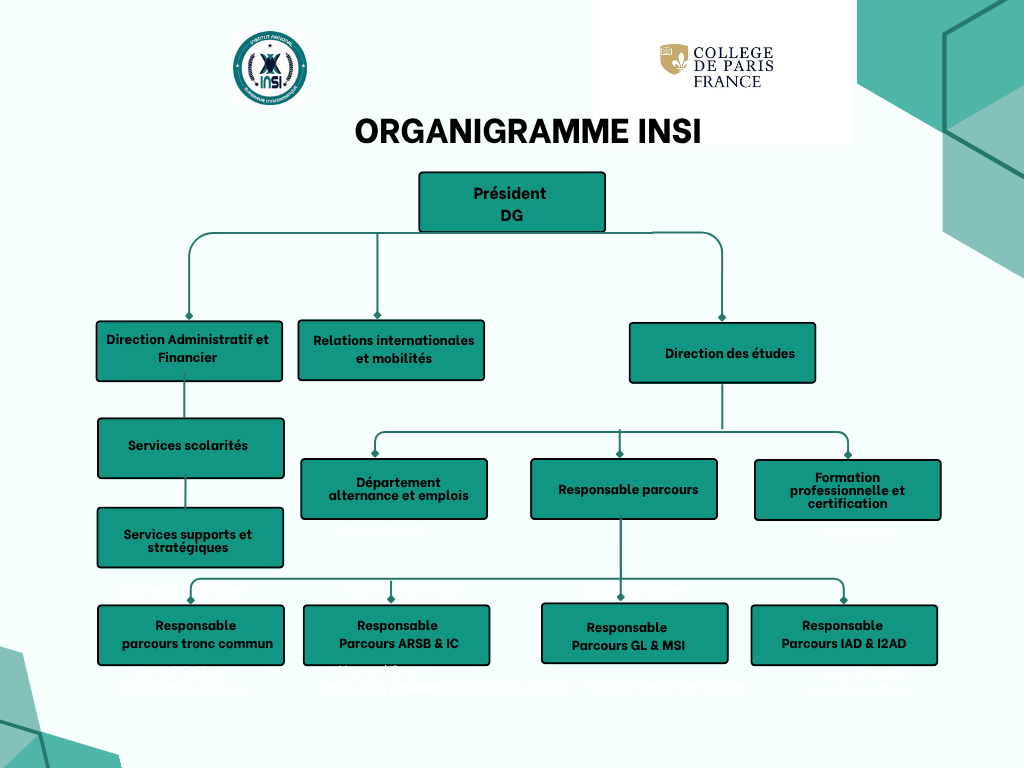
\includegraphics[width=6.89375in,height=5.86389in]{../figures/image1.png}

\textbf{Figure 1~: Organigramme de l'INSI}

L\textquotesingle organigramme de l'INSI, en partenariat avec le Collège
de Paris, est structuré autour d'une direction générale incarnée par le
Président Directeur Général. Ce dernier assure la coordination de trois
pôles principaux : la Direction Administrative et Financière, la
Direction des Études, et le service des Relations Internationales et
Mobilités.

Le Président Directeur Général assure la direction
stratégique de l'institut. Il supervise l'ensemble des activités
pédagogiques, administratives et de développement.

Il veille à la qualité de l'enseignement, à la bonne gestion des
ressources humaines et matérielles, et représente l'établissement auprès
des partenaires et autorités.

La Direction Administrative et Financière est chargée de la
gestion des affaires internes, notamment à travers deux services
essentiels : le service des scolarités, qui s'occupe des
dossiers étudiants, inscriptions et suivi académique, et les
services supports et stratégiques, qui assurent un appui
logistique, administratif et technologique à l'ensemble de l'institut.

Le pôle des Relations Internationales et Mobilités gère les
échanges académiques avec l'étranger ainsi que les projets de mobilité
étudiante ou enseignante.

La Direction des Études supervise quant à elle l'ensemble des
programmes pédagogiques et le corps enseignant. Elle travaille en
étroite collaboration avec un Responsable Parcours, qui
coordonne les différentes spécialisations proposées. Cette direction
intègre également une cellule dédiée à la formation
	professionnelle et à la certification, en charge des dispositifs de
validation des compétences, des certifications professionnelles et des
parcours de formation continue. Il comprend également le
Département alternance et emplois, responsable du suivi des
étudiants en contrat d'alternance, des stages professionnels, et de
l'insertion professionnelle.

Sous la partie Responsable Parcours, plusieurs responsables
pédagogiques gèrent les différentes filières de formation : le
parcours tronc commun, qui regroupe les matières fondamentales
partagées par tous les étudiants en début de cycle ; le parcours
	ARSB \& IC; le parcours GL \& MSI ; et enfin le
parcours IAD \& I2AD.

D'autres structures, bien que non représentés sur cet organigramme,
contribuent également de manière significative à la mission de l'INSI.

Le Conseil de l'École, Il regroupe des membres de l'équipe
pédagogique et administrative. Il joue un rôle consultatif ou
décisionnel sur les questions académiques : validation des programmes,
suivi des résultats, discipline, méthodologie, etc.

Le responsable de la formation en ligne, Il conçoit et
supervise les dispositifs d'apprentissage à distance. Il s'assure que
les contenus en ligne sont accessibles, interactifs et conformes aux
standards pédagogiques, tout en accompagnant enseignants et étudiants
dans leur utilisation.

L'Association et Clubs étudiants, encadre et soutient les
initiatives étudiantes, les clubs thématiques (informatique, innovation,
sport, culture, etc.), et les événements organisés dans le cadre de la
vie étudiante. Cela favorise l'engagement, le développement personnel et
les compétences transversales des étudiants.

Cette structure témoigne d'une organisation à la fois pédagogique,
administrative et tournée vers l'international et l'employabilité,
assurant une formation complète et professionnalisante aux étudiants.

\begin{enumerate}
	\def\labelenumi{\arabic{enumi}.}
	\setcounter{enumi}{1}
	\item
	\textbf{Domaine de spécialisation}
\end{enumerate}

INSI University propose des parcours académiques
	professionnalisants dans le domaine de l'informatique et des
technologies numériques, articulés autour de licences professionnelles,
de masters spécialisés, formations professionnelles continues et
d'opportunités de mobilité internationale.

\begin{enumerate}
	\def\labelenumi{\alph{enumi})}
	\item
	\textbf{\uline{Licences professionnelles}}
\end{enumerate}

Les programmes de licence offrent une formation de base solide, axée sur
la pratique, et préparant à une insertion rapide dans le monde
professionnel :

GL (Génie Logiciel) : Conception, développement et maintenance
d\textquotesingle applications logicielles.

ARSB (Administration Réseaux et Systèmes et Base de données) :
Gestion d'infrastructures informatiques, réseaux, serveurs et systèmes.

IAD (Intelligence Artificielle et Data Science) : Introduction
aux algorithmes d'IA, au traitement de données et à l'apprentissage
automatique.

\begin{enumerate}
	\def\labelenumi{\alph{enumi})}
	\setcounter{enumi}{1}
	\item
	\textbf{\uline{Masters professionnels}}
\end{enumerate}

Les masters permettent d'approfondir les compétences techniques et
managériales, en lien étroit avec les évolutions du secteur :

MSI (Management des Systèmes d'Information) : Pilotage de
projets numériques, gouvernance des SI.

IC (Infrastructures et Cybersécurités) : Sécurisation des
systèmes, audit, réseaux avancés.

IAD (Intelligence Artificielle, Analyse de Données et
	Automatisation) : Applications avancées de l'IA, automatisation des
processus et science des données.

\begin{enumerate}
	\def\labelenumi{\alph{enumi})}
	\setcounter{enumi}{2}
	\item
	\textbf{Formations professionnelles}
\end{enumerate}

INSI University propose également des formations professionnelles
continues, spécifiquement conçues pour les professionnels déjà en poste
souhaitant approfondir leurs compétences ou se spécialiser dans l'un des
domaines proposés.\\
Ces formations sont adaptées aux contraintes des professionnels
(horaires flexibles, modules pratiques) et visent à renforcer leur
employabilité ou à accompagner leur évolution de carrière.

\begin{enumerate}
	\def\labelenumi{\alph{enumi})}
	\setcounter{enumi}{3}
	\item
	\textbf{Mobilité internationale \& double diplôme}
\end{enumerate}

Dans une optique d'ouverture et de reconnaissance internationale, INSI
propose à ses étudiants des opportunités de mobilité académique et de
double diplôme, à partir de la deuxième année (L2).

\begin{itemize}
	\item
	\textbf{Format hybride} : \emph{6 mois de formation à Madagascar + 6
		mois à l'étranger} selon le parcours choisi.
\end{itemize}

\begin{itemize}
	\item
	\textbf{Double diplôme en L3 ou M2} : En partenariat avec des
	institutions internationales telles que :
	
	\begin{itemize}
		\item
		Collège de Paris (France)
	\end{itemize}
	
	\begin{itemize}
		\item
		Keyce Informatique (France)
	\end{itemize}
	
	\begin{itemize}
		\item
		Eskills (Québec, Canada)
	\end{itemize}
\end{itemize}

\hypertarget{conditions-duxe9ligibilituxe9}{%
	\paragraph{\texorpdfstring{\textbf{Conditions
				d'éligibilité}}{Conditions d'éligibilité}}\label{conditions-duxe9ligibilituxe9}}

\begin{itemize}
	\item
	Niveau DALF C1 en français pour la mobilité vers des pays
	francophones.
	\item
	Niveau B2 ou C1 en anglais pour les destinations anglophones.
	
	\begin{enumerate}
		\def\labelenumi{\arabic{enumi}.}
		\item
		Architectures des formations pédagogiques
	\end{enumerate}
\end{itemize}

Le recrutement des étudiants à l'INSI s'effectue exclusivement par
sélection de dossiers pour l'entrée en première année de Licence (L1),
et par voie de concours pour l'admission en Master 1,

Au sein de l'INSI, une seule mention est proposée : Informatique,
déclinée en trois parcours distincts aux niveaux Licence et Master :

Tableau 1~: Les parcours en Licence et Master

\begin{table}[H]
	\centering
	\begin{tabular}{|p{7cm}|p{7cm}|}
		\hline
		\textbf{Licence} & \textbf{Master} \\
		\hline
		Génie Logiciel (GL) & Management des Systèmes d’Information (MSI) \\
		\hline
		Administration Réseaux, Systèmes et Bases de données (ARSB) & Infrastructures et Cybersécurités (IC) \\
		\hline
		Intelligence Artificielle et Data Science (IAD) & Intelligence Artificielle, Analyse de Données et Automatisation (I2AD) \\
		\hline
	\end{tabular}
	\caption{Exemple de parcours Licence/Master}
\end{table}


L'architecture des études à trois niveaux conformément au système LMD
(Licence Master et Doctorat) permet les comparaisons et les équivalences
académiques des diplômes au niveau international.

L = Licence (Bac + 3) = L1, L2, L3 = 6 semestres S1 à S6

M = Master (Bac + 5) = M1, M2 = 4 \textbf{semestres S7 à S10}

Le diplôme de licence est obtenu en 3 années des études après
Baccalauréat. Et le

diplôme de Master est obtenu en 2 ans après obtenu du diplôme de
LICENCE.

Le MASTER PROFESSIONNEL est un diplôme destiné à la recherche emploi au
terme

des études.

\textbf{Spécificités pédagogiques}

\begin{itemize}
	\item
	\textbf{École d\textquotesingle alternance dès la L2 S4}\\
	Alternance cours/entreprise pour une meilleure insertion
	\item
	\textbf{Écoles connectées \& e-learning}\\
	Plateforme numérique de formation, cloud intégré, Google Workspace\\
	Cours accessibles en ligne selon les parcours
	\item
	\textbf{Pédagogie active \& par projets\\
		Hackathons, soutenances exposées, projets réels en entreprise}
	
	\begin{enumerate}
		\def\labelenumi{\arabic{enumi}.}
		\item
		\textbf{Relations de l'INSI avec les entreprises et les organismes}
	\end{enumerate}
\end{itemize}

L'Institut National Supérieur en Informatique (INSI) entretient des
liens étroits avec le monde professionnel. L'INSI collabore activement
avec de nombreux organismes publics, semi-publics et privés, tant au
niveau national qu'international. Cette collaboration se traduit
concrètement par l'organisation régulière de stages obligatoires pour
les étudiants, favorisant leur immersion professionnelle et leur
employabilité.

Parmi les entreprises et institutions partenaires accueillant nos
étudiants en stage chaque année, on peut citer : Data Pulse Center,
RELIA Consulting, Code Talent, Bocasay, Minimad, Smartone AI, NOVITY,
Eclosia Madagascar, VISEO Groupe, Océane Trade, ACCES Banque, ...

En plus des stages, l'INSI organise régulièrement des visites
	pédagogiques, des rencontres métiers et des projets
	collaboratifs avec plusieurs entreprises du secteur technologique et
numérique. Ces activités permettent aux étudiants de mieux comprendre
les réalités du terrain, d'échanger avec des professionnels et de
s'ouvrir à l'environnement entrepreneurial.

Parmi les entreprises ayant accueilli ces initiatives : NOVITY, YAS
Madagascar, Smartone AI, Eclosia Madagascar, et d\textquotesingle autres
acteurs majeurs du numérique à Madagascar.

Cette dynamique de partenariat permanent constitue un pilier de la
pédagogie à l'INSI, en lien avec son objectif de former des
professionnels compétents, opérationnels et ancrés dans les besoins du
marché.

\begin{enumerate}
	\def\labelenumi{\arabic{enumi}.}
	\setcounter{enumi}{1}
	\item
	\textbf{Partenariat au niveau international}
\end{enumerate}

L'INSI s'est inscrit dans une dynamique d'ouverture à l'international
grâce à son partenaire fondateur, ILO Madagascar, représentant
de l'Organisation Internationale du Travail. Cette orientation se
renforce aujourd'hui à travers des partenariats stratégiques
	avec des institutions académiques et des entreprises internationales,
permettant à l'Institut de proposer une formation alignée sur les
standards mondiaux.

L'INSI bénéficie actuellement de programmes de co-diplomation et
	de double diplôme en collaboration avec plusieurs établissements
internationaux de renom, tels que :

\begin{itemize}
	\item
	\textbf{Collège de Paris International}
	\item
	\textbf{Keyce Informatique} (France)
	\item
	\textbf{Eskills Academy} (Québec, Canada)
	\item
	\textbf{École Supérieure Polytechnique d'Antsiranana (ESPA)} -- pour
	une synergie régionale renforcée.
\end{itemize}

Ces partenariats permettent non seulement d'enrichir l'offre
pédagogique, mais aussi d'ouvrir des perspectives de mobilité
	académique et professionnelle aux étudiants, en leur offrant
une reconnaissance de leurs compétences à l'échelle internationale.

Par ailleurs, à travers les stages annuels et projets
	pédagogiques, l'INSI collabore également avec des entreprises à
dimension régionale ou mondiale, telles que :

\begin{itemize}
	\item
	\textbf{VISEO Groupe}
	\item
	\textbf{Eclosia Madagascar} (Groupe mauricien)
	\item
	\textbf{Smartone AI}
	\item
	\textbf{NOVITY}, entre autres.
\end{itemize}

Ces relations actives témoignent de l'ancrage de l'INSI dans un
écosystème global, plaçant l'Institut comme un acteur majeur de
la formation en informatique à Madagascar, tourné vers l'innovation et
les exigences du marché international.

\begin{enumerate}
	\def\labelenumi{\arabic{enumi}.}
	\item
	\textbf{Parcours professionnels des diplômés}
\end{enumerate}

Les diplômés de la Licence en Informatique de l'INSI disposent d'un
socle solide de compétences en programmation, systèmes, réseaux, bases
de données et développement logiciel. Cette polyvalence leur permet
d'intégrer directement le marché du travail ou de poursuivre en Master.
À ce niveau, ils peuvent exercer en tant que :

\begin{itemize}
	\item
	\textbf{Technicien système et réseau}
	\item
	\textbf{Développeur web / mobile (front-end ou back-end)}
	\item
	\textbf{Administrateur systèmes junior}
	\item
	\textbf{Technicien support IT}
	\item
	\textbf{Intégrateur / testeur logiciel}
	\item
	\textbf{Assistant en sécurité informatique}
	\item
	\textbf{Assistant en projets d'IA ou de data (selon profil)}
\end{itemize}

Les stages annuels en entreprise leur offrent une première expérience
professionnelle valorisante dans des structures variées : entreprises
technologiques, banques, administrations, startups, ONG, etc.

La formation de Master proposée à l'INSI, grâce à ses parcours
spécialisés, forme des professionnels capables d'intervenir sur des
projets complexes, innovants et à dimension stratégique. Les débouchés
varient selon la spécialisation choisie :

\hypertarget{parcours-inguxe9nierie-logicielle-ruxe9seaux-et-systuxe8mes}{%
	\subparagraph{Parcours Ingénierie logicielle, réseaux et systèmes
		:}\label{parcours-inguxe9nierie-logicielle-ruxe9seaux-et-systuxe8mes}}

\begin{itemize}
	\item
	\textbf{Ingénieur en développement logiciel / full-stack}
	\item
	\textbf{Architecte logiciel}
	\item
	\textbf{Ingénieur systèmes et réseaux}
	\item
	\textbf{Administrateur cloud / DevOps}
	\item
	\textbf{Chef de projet informatique}
\end{itemize}

\hypertarget{parcours-cybersuxe9curituxe9}{%
	\subparagraph{Parcours Cybersécurité
		:}\label{parcours-cybersuxe9curituxe9}}

\begin{itemize}
	\item
	\textbf{Expert en sécurité des systèmes d\textquotesingle information}
	\item
	\textbf{Analyste SOC / CERT}
	\item
	\textbf{Auditeur en cybersécurité}
	\item
	\textbf{Responsable de la sécurité IT (RSSI)}
\end{itemize}

\hypertarget{parcours-intelligence-artificielle-et-data}{%
	\subparagraph{Parcours Intelligence Artificielle et Data
		:}\label{parcours-intelligence-artificielle-et-data}}

\begin{itemize}
	\item
	\textbf{Data Scientist}
	\item
	\textbf{Data Analyst}
	\item
	\textbf{Ingénieur en Intelligence Artificielle}
	\item
	\textbf{Machine Learning Engineer}
	\item
	\textbf{Développeur d\textquotesingle applications intelligentes}
	\item
	\textbf{Consultant en IA}
	\item
	\textbf{Spécialiste en traitement automatique du langage naturel
		(TALN)}
	\item
	\textbf{Spécialiste en vision par ordinateur (Computer Vision)}
\end{itemize}

Grâce aux partenariats internationaux et aux projets en
	entreprise, les diplômés du Master peuvent également prétendre à des
postes dans des structures multinationales, ou poursuivre une
carrière académique et de recherche (doctorat, enseignement
supérieur).

\begin{enumerate}
	\def\labelenumi{\arabic{enumi}.}
	\item
	\textbf{Ressources humaines}
\end{enumerate}

L'INSI s'appuie sur une équipe pédagogique et administrative compétente,
dynamique et engagée dans la réussite de ses étudiants. Ses ressources
humaines se répartissent comme suit :

Président Directeur de l'INSI~: Dr RAMASONDRANO Andriamanjaka

Responsable parcours~ARSB \& IC~: Mr RATIANARISON Hery Mampionona

Responsable parcours tronc commun : Dr RAKOTONDRAMANANA R, Sitraka

Responsable parcours GL \& MSI~: Mr ANDRIAMIADANA TANTELY ANTOINE

Responsable parcours IAD \& I2AD~: par intérim PDG

Nombres des enseignants : 40

Nombres des personnels administratives : 04

Personnels d'appui~: 6


>>>>>>> 7f1856b (Ajustement du livre)
\begin{titlepage}
    \centering
    \vspace*{\fill} % centre verticalement
    {\Huge \textbf{Prediciton du taux de reussite au concours d’entré école/université} \par}
    \vspace{2cm}
    {\Large Auteur : Aritendry RAMAHAFENO et Bernardin RASOLONJANAHARY \par}
    \vspace*{\fill}
\end{titlepage}

\chapter*{Remerciements}
\addcontentsline{toc}{chapter}{Remerciements}

D'abord, on veut vraiment dire merci à Dieu qui nous a accompagnés pendant tout ce projet de fin d'études. Sans Sa grâce, on aurait pas eu la force ni le courage d'aller au bout.

On tient aussi à remercier le Dr Dimby qui nous a supervisés. Ses conseils et sa disponibilité ont été super précieux pour nous, surtout quand on bloquait sur certains points.

Un grand merci aussi à tous les profs du département d'Informatique de l'INSI. Les cours qu'on a eus pendant les deux semestres nous ont vraiment préparés pour ce projet.

Et pour finir, merci du fond du cœur à nos familles. Leur soutien et leurs encouragements ont été super importants pour nous, surtout dans les moments un peu difficiles.
\chapter*{Résumé}
\addcontentsline{toc}{chapter}{Résumé}

Dans ce travail de fin d'études, on s'est penché sur la prédiction des chances de réussite aux concours d'entrée à l'université. On est parti d'un jeu de données avec différentes variables académiques - les scores GRE et TOEFL, la moyenne générale CGPA, et quelques autres critères qui peuvent jouer.

Le boulot a consisté d'abord à nettoyer et préparer ces données, puis à tester plusieurs approches de modélisation. Finalement, on a opté pour une forêt aléatoire (Random Forest) qui semblait donner les meilleurs résultats pour prédire l'admission des candidats.

Les résultats sont plutôt bons, avec une précision qui dépasse 90% sur nos tests. Ça montre que les critères qu'on a choisis sont effectivement pertinents pour ce type de prédiction. À l'avenir, ce travail pourrait servir de base pour développer des outils d'aide à la décision, autant pour les étudiants que pour les établissements.

\chapter*{Abstract}
\addcontentsline{toc}{chapter}{Abstract}

This final year project tackles the prediction of success rates in university entrance exams. We worked with a dataset containing various academic indicators including GRE and TOEFL scores, CGPA, and other relevant factors that might influence admission chances.

The work involved cleaning and preparing the data, then experimenting with different modeling approaches. We ultimately selected a Random Forest classifier which showed the best performance in predicting candidate admission.

The results are quite encouraging, with accuracy exceeding 90% in our tests. This demonstrates that the chosen variables are indeed relevant for this type of prediction. In the future, this work could serve as a foundation for developing decision support tools for both students and educational institutions.

\clearpage
\tableofcontents
\newpage

% ------------ Import des fichiers ------------
\pagenumbering{arabic}
\chapter{Introduction Générale}

\section{Contexte}

L’entrée à l’université représente un enjeu important pour beaucoup d’étudiants, et les concours d’admission sont souvent une étape décisive. Pouvoir prédire les chances de réussite permet non seulement d’aider les candidats à mieux se préparer, mais aussi d’accompagner les établissements dans leur processus de sélection.

\section{Problématique}

Prédire si un candidat va réussir son concours d’entrée est un vrai défi : les données sont nombreuses, variées, et pas toujours très propres. Difficile, dans ces conditions, de bâtir un modèle fiable. Il fallait donc trouver une manière efficace de traiter ces informations pour en tirer des prédictions utiles.

\section{Objectifs}

L’objectif de ce projet était de développer un modèle capable d’estimer les probabilités de réussite au concours, en se basant sur des données académiques comme les scores au GRE ou au TOEFL, la moyenne générale, et d’autres critères pertinents.

\section{Démarche suivie}

Pour y parvenir, on a commencé par rassembler plusieurs jeux de données, puis on en a choisi un — le plus complet et fiable. Ensuite, on a nettoyé et préparé les données, avant de les explorer pour bien comprendre ce qu’elles contenaient. Plusieurs algorithmes de machine learning ont été testés et comparés pour sélectionner celui qui donnait les meilleurs résultats.

\section{Structure du rapport}

Ce mémoire est organisé en quatre parties : 
\begin{itemize}
    \item La première partie présente la collecte et le prétraitement des données.
    \item La deuxième détaille la modélisation et l’évaluation des différents algorithmes.
    \item La troisième analyse les résultats et les performances du modèle retenu.
    \item Enfin, la dernière partie discute des limitations et propose des pistes d’amélioration pour aller plus loin.
\end{itemize}
\section{Exploration des données}

\subsection{Chargement du jeu de données}

Le jeu de données  a été chargé au format .CSV à l’aide de la bibliothèque python \texttt{pandas} :

\begin{verbatim}
import pandas as pd
df = pd.read_csv("admission_data.csv")
\end{verbatim}

La commande \texttt{df.info()}permet de voir une partie des colonnes, de leurs types et du nombre de valeurs non nulles. On compte 9 colonnes et 550 lignes.

\subsection{Aperçu des données}

\begin{itemize}
    \item Le jeu de données contient des variables quantitatives comme par exemple (\textit{GRE Score}, \textit{TOEFL Score}, \textit{CGPA}, \textit{Chance of Admit}) et discrètes (\textit{University Rating}, \textit{SOP}, \textit{LOR}, \textit{Research}).
    \item Ici \textit{Chance of Admit} est la variable cible. Elle indique la probabilité d’admission.
\end{itemize}

\subsection{Traitement des valeurs manquantes}

Des valeurs manquantes ont été détectées dans deux colonnes :
\begin{itemize}
    \item \textbf{TOEFL Score}
    \item \textbf{SOP (Statement of Purpose)}
\end{itemize}

Ces deux colonnes présentaient chacune 37 valeurs manquantes.

La stratégie choisie a été de supprimer toutes les lignes contenant au moins une valeur manquante :

\begin{verbatim}
df_clean = df.dropna()
\end{verbatim}

Puis on a fait une vérification pour s'il n'y a plus de variable manquantes dans le dataset

\begin{verbatim}
df_clean.isnull().sum()
\end{verbatim}

Résultat : toutes les valeurs manquantes ont été supprimées. Le jeu de données final contient 513 lignes.

\subsection{Détection de doublons}

Pour vérifier la présence de doublons, j’ai utilisé la commande suivante :

\begin{verbatim}
df_clean.duplicated().sum()
\end{verbatim}

Résultat : aucune ligne dupliquée n’a été détectée.

\subsection{Étude des valeurs aberrantes}

Des diagrammes en boîte (\textit{boxplots}) ont été tracés pour les variables numériques afin de visualiser les potentiels outliers. Bien que certains points soient situés à l’extérieur du graphe de boites a moustache, aucun n’a été jugé significativement aberrant ou incohérent (par exemple, un CGPA supérieur à 10 ou un score GRE supérieur à 340). Aucun traitement particulier n’a été effectué à ce niveau.

\subsection{Étude des corrélations}

Une matrice de corrélation a été générée pour évaluer les relations entre les variables :

\begin{verbatim}
corr_matrix = df_clean.corr()
\end{verbatim}

Les coefficients de corrélation les plus élevés avec la variable cible \textit{Chance of Admit} sont :
\begin{itemize}
    \item \textbf{CGPA} : 0.87
    \item \textbf{GRE Score} : 0.82
    \item \textbf{TOEFL Score} : 0.79
    \item \textbf{Research} : 0.55
\end{itemize}

On voit que les performances académiques (CGPA, GRE, TOEFL) et l'expérience de recherche sont fortement corrélés aux chances d'admission.

\subsection{Conclusion de l'exploration}

L'analyse exploratoire a permis de :
\begin{itemize}
    \item Nettoyer le jeu de données (suppression des lignes incomplètes),
    \item Confirmer l'absence de doublons,
    \item Identifier les variables les plus corrélées à la cible,
    \item Préparer les données pour les étapes de visualisation et de modélisation.
\end{itemize}
         % EDA
\section{Présentation des dataset secondaires}

\textbf{Nom du Dataset :} gc\_data.csv

\vspace{0.5cm}
\textbf{Les colonnes du dataset :}
\begin{itemize}
	\item School, Program, Result, Result\_Date, GPA, 
	\item Verbal\_GRE, Quant\_GRE, Writing\_GRE, Subject\_GRE, 
	\item Status, Submit\_Date, Degree\_Type
\end{itemize}

\vspace{0.5cm}
\textbf{Aperçu des 5 premières lignes du dataset :}

\begin{center}
	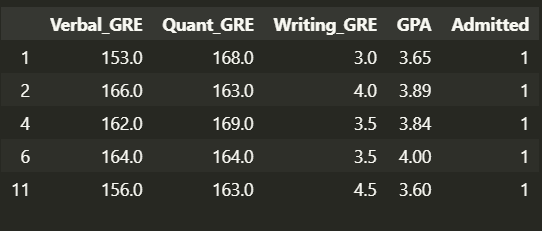
\includegraphics[width=0.9\textwidth]{../figures/head.png}
	\captionof{figure}{Aperçu des 5 premières lignes du dataset}
\end{center}

\begin{center}
	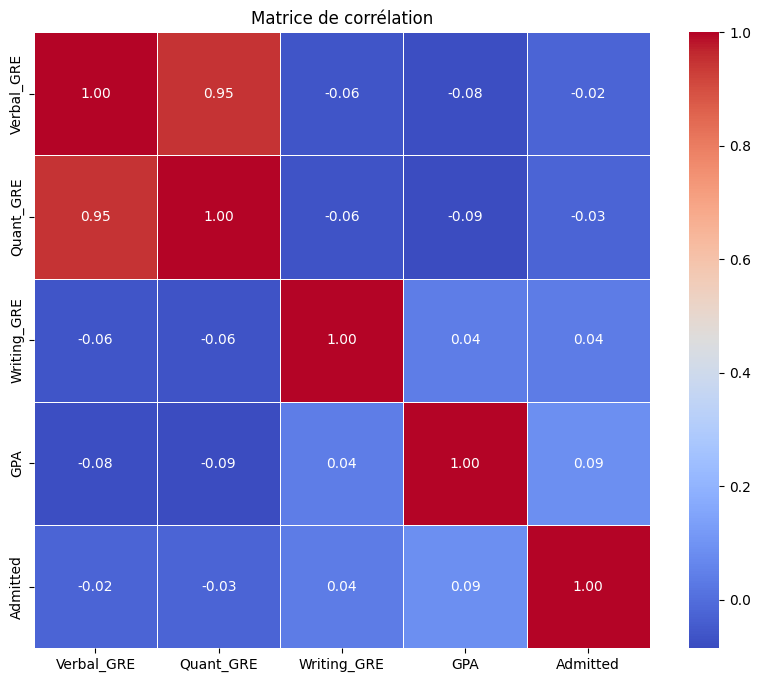
\includegraphics[width=0.9\textwidth]{../figures/corr.png}
\end{center}

Les variables principales du dataset secondaire \textbf{gc\_data.csv} (Verbal\_GRE, Quant\_GRE, Writing\_GRE et GPA) sont faiblement corrélées à la variable cible (\textbf{Admitted}). Cette faiblesse de corrélation peut être due à une falsification des données.

\vspace{0.5cm}
\textbf{Choix des variables explicatives (X) :} \\
Nous avons sélectionné les variables suivantes comme variables explicatives :
\begin{itemize}
	\item Verbal\_GRE
	\item Quant\_GRE
	\item Writing\_GRE
	\item GPA
	\item Admitted
\end{itemize}

\vspace{0.3cm}
\textbf{Variable cible (Y) :} \\
La variable cible est \textbf{Admitted}. Cette variable correspond à notre objectif d'étude, car elle représente la classification binaire : 1 pour admit et 0 pour le contraire, permettant de prédire si l'étudiant peut être admis ou non.

\textbf{Nom du Dataset :} Australian\_Student\_PerformanceData (ASPD24).csv \\
Ce dataset contient des données de performance des étudiants australiens.

\vspace{0.5cm}
\textbf{Les colonnes dans le dataset :}
\begin{itemize}
	\item 51 colonnes, y compris :
	\begin{itemize}
		\item GPA
		\item High School GPA
		\item Entrance Exam Score
		\item Attendance
		\item Family Income
		\item Parental Education
		\item Health
		\item Mental Health
		\item Exam Scores
		\item Final Exam Scores
		\item Gender
		\item Hours of Study per Week
		\item Performance ou P\_encoded après l'encodage de la variable cible
	\end{itemize}
\end{itemize}


\vspace{0.5cm}
\textbf{Aperçu des 5 premières lignes du dataset :}

\begin{center}
	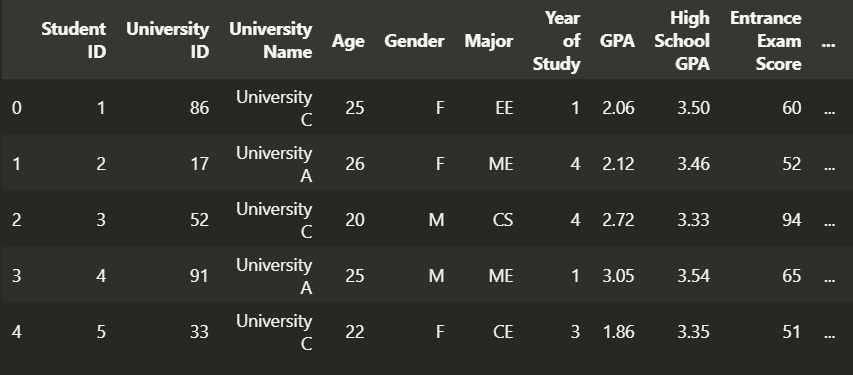
\includegraphics[width=0.9\textwidth]{../figures/head1.png}
	\captionof{figure}{Les 5 premières lignes du dataset}
\end{center}

Les variables indépendantes suivantes : GPA, High School GPA, Entrance Exam Score, Attendance, Family Income, Parental Education, Health, Mental Health, Exam Scores sont peu corrélées à la variable cible (\textbf{Performance} ou \textbf{P\_encoded}), comme le montre la figure ci-dessous.

\begin{figure}[!htbp]
	\centering
	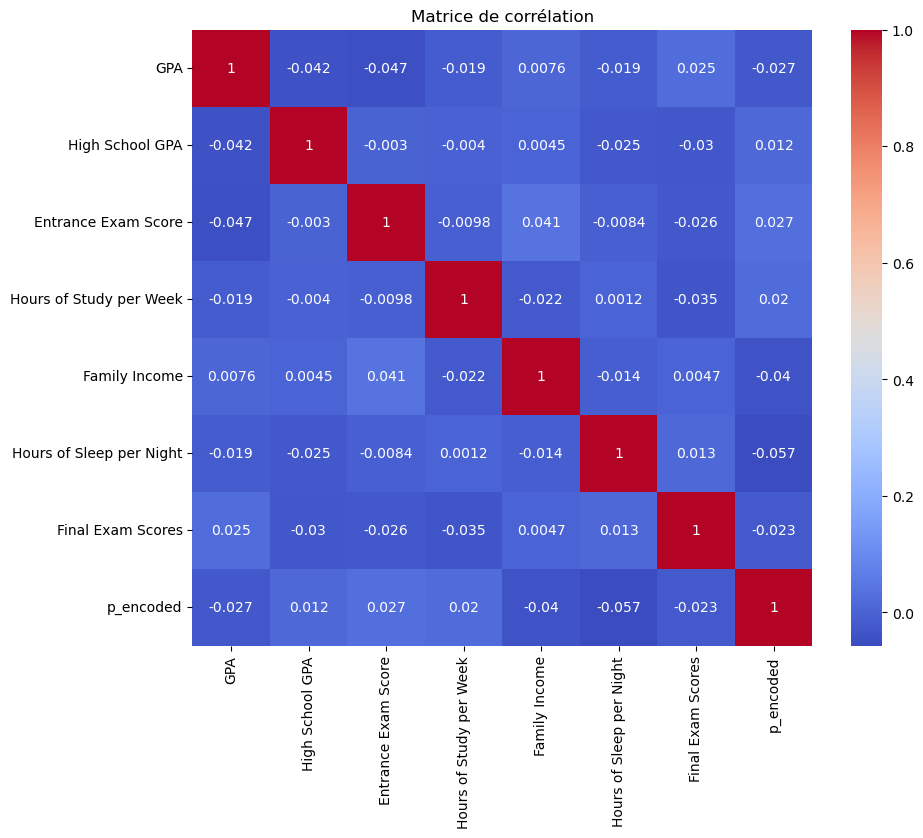
\includegraphics[width=0.9\textwidth]{../figures/corr1}
	\caption{}
	\label{fig:corr1}
\end{figure}

\vspace{0.5cm}
\textbf{Choix des variables explicatives (X) :} \\
Parmi les variables ci-dessus, nous avons sélectionné les variables suivantes :
\begin{itemize}
	\item GPA
	\item Final Exam Scores
	\item Gender
	\item Parental Education Level
	\item Family Income
	\item Hours of Study per Week
\end{itemize}

\vspace{0.3cm}
\textbf{Variable cible (Y) :} \\
La variable cible est \textbf{Performance} ou \textbf{P\_encoded}. Elle correspond à environ 70\% de notre objectif d'étude, car elle représente la performance des étudiants mais pas exactement la classification.

\section{Visualisation des données du dataset principal}

\section{Analyse univariée}

\subsection{GRE Score}
Pour analyser la distribution du GRE Score, nous avons utilisé un histogramme (\textbf{Figure 1.4}).

\begin{figure}[!htbp]
	\centering
	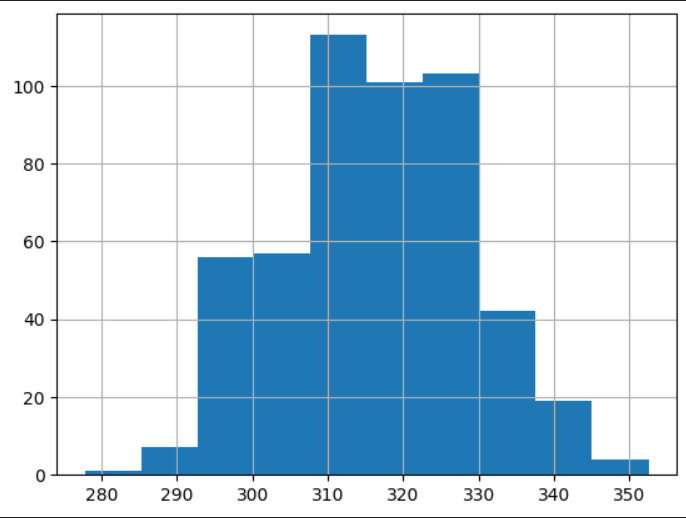
\includegraphics[width=0.9\textwidth]{../figures/hist_gre_score.png}
	\caption{Distribution du GRE Score}
	\label{fig:hist_gre_score}
\end{figure}

La majorité des scores GRE se situe entre 300 et 335, montrant une répartition homogène avec une concentration autour de scores élevés.

\subsection{CGPA}
Distribution du CGPA (\textbf{Figure 1.5}).

\begin{figure}[!htbp]
	\centering
	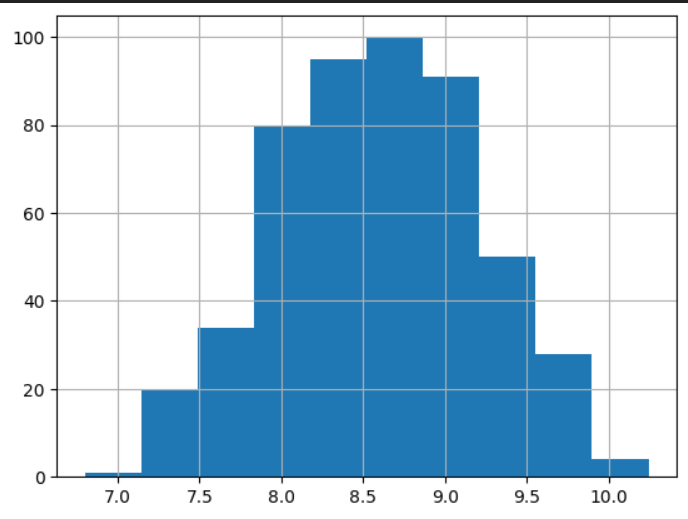
\includegraphics[width=0.9\textwidth]{../figures/hist_cgpa.png}
	\caption{Distribution du CGPA}
	\label{fig:hist_cgpa}
\end{figure}

La majorité des CGPA sont entre 8.0 et 9.5, peu de candidats en dessous de 7.5.

\subsection{TOEFL Score}
Distribution du TOEFL Score (\textbf{Figure 1.6}).

\begin{figure}[!htbp]
	\centering
	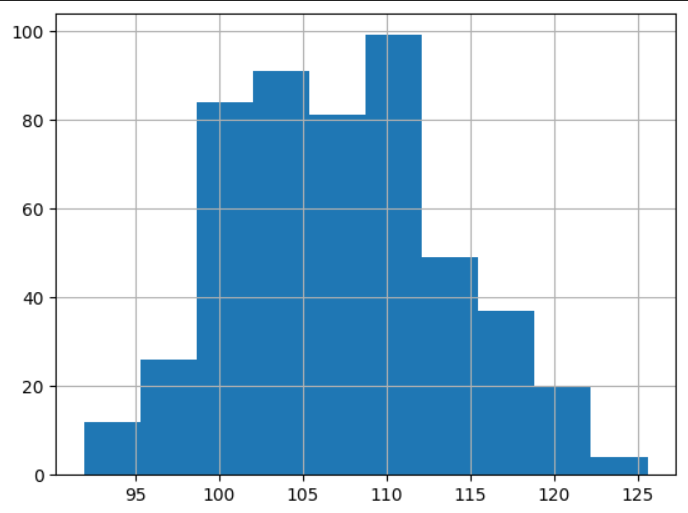
\includegraphics[width=0.9\textwidth]{../figures/hist_toefl_score.png}
	\caption{Distribution du TOEFL Score}
	\label{fig:hist_toefl_score}
\end{figure}

Les scores se concentrent entre 100 et 110, avec quelques candidats dépassant 115.

\subsection{University Rating}
Distribution de University Rating (\textbf{Figure 1.7}).

\begin{figure}[!htbp]
	\centering
	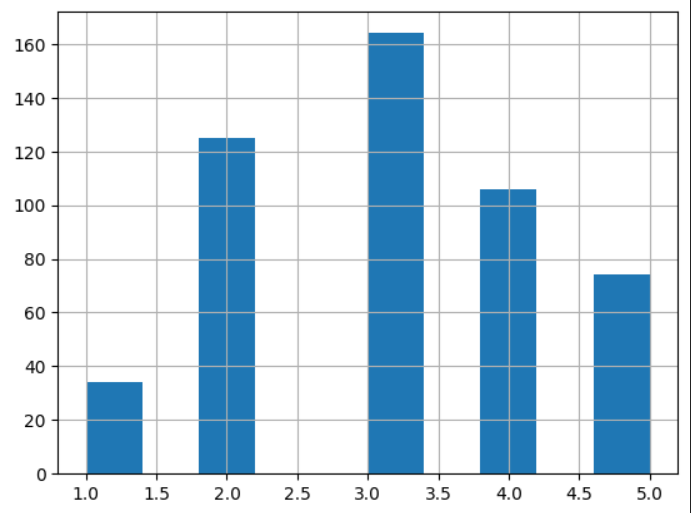
\includegraphics[width=0.9\textwidth]{../figures/hist_university_rating.png}
	\caption{Distribution de l'évaluation des universités}
	\label{fig:hist_university_rating}
\end{figure}

Les notes sont principalement entre 2 et 4.

\subsection{Research}
Répartition des étudiants selon expérience de recherche (\textbf{Figure 1.8}).

\begin{figure}[!htbp]
	\centering
	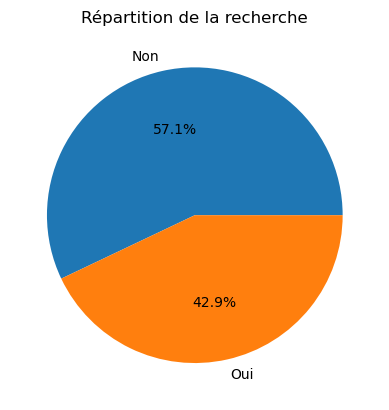
\includegraphics[width=0.9\textwidth]{../figures/pie.png}
	\caption{Répartition des candidats selon l’expérience de recherche}
	\label{fig:pie_research}
\end{figure}

57.1\% ont une expérience de recherche contre 42.9\% qui n’en ont pas.

\subsection{Chance of Admit}
Distribution de la probabilité d’admission (\textbf{Figure 1.9}).

\begin{figure}[!htbp]
	\centering
	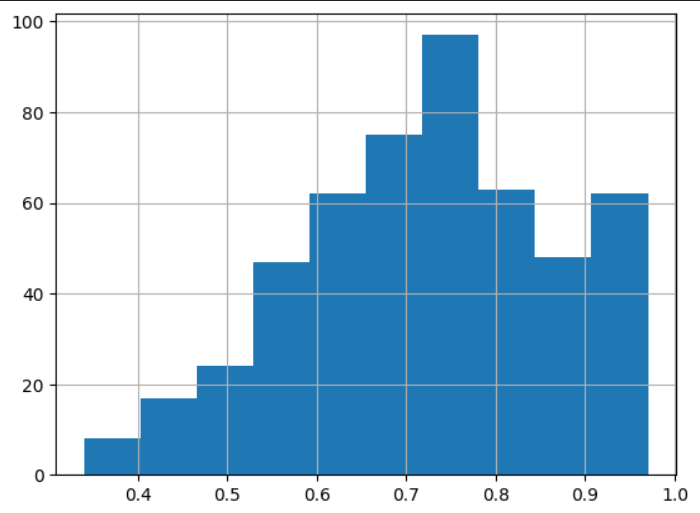
\includegraphics[width=0.9\textwidth]{../figures/hist_chance_admit.png}
	\caption{Distribution de la probabilité d’admission}
	\label{fig:hist_chance_admit}
\end{figure}

La majorité des valeurs se situe entre 0.6 et 0.8, avec une deuxième concentration entre 0.8 et 0.9.

\section{Analyse bivariée}

\subsection{GRE Score vs Chance of Admit}
Nuage de points (\textbf{Figure 1.10}).

\begin{figure}[!htbp]
	\centering
	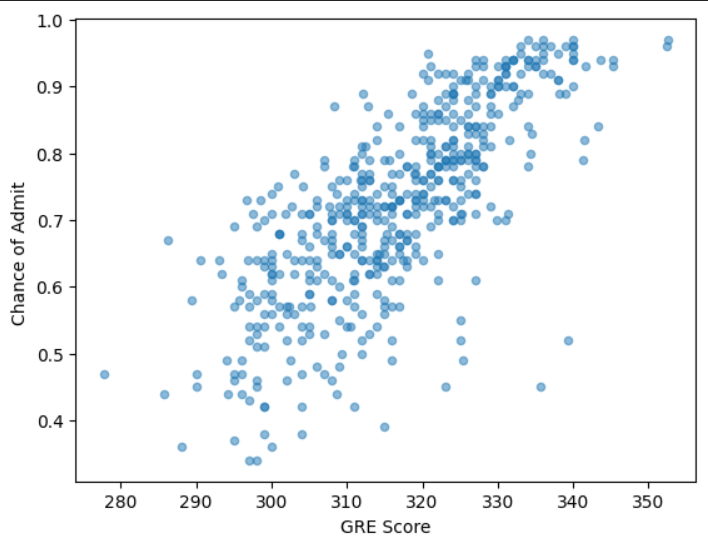
\includegraphics[width=0.9\textwidth]{../figures/scatter_gre_admit.png}
	\caption{Relation entre GRE Score et Chance of Admit}
	\label{fig:scatter_gre_admit}
\end{figure}

Relation croissante : GRE > 320 → plus de chances d’admission.

\subsection{CGPA vs Chance of Admit}
Nuage de points (\textbf{Figure 1.11}).

\begin{figure}[!htbp]
	\centering
	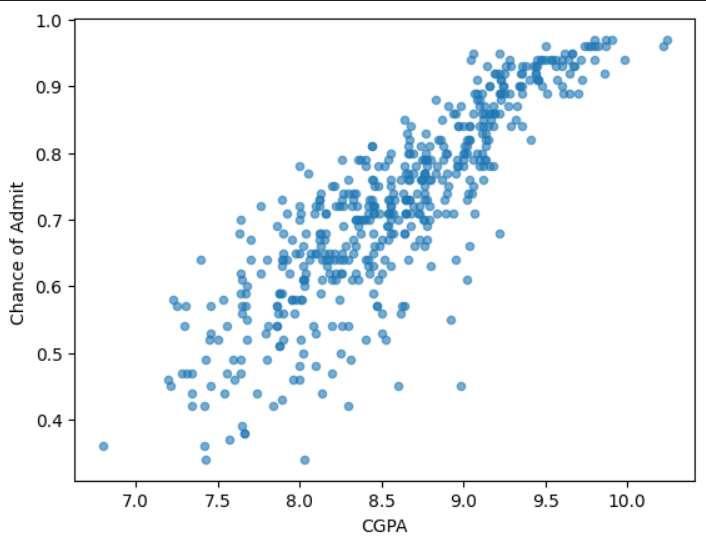
\includegraphics[width=0.9\textwidth]{../figures/scatter_cgpa_admit.png}
	\caption{Relation entre CGPA et Chance of Admit}
	\label{fig:scatter_cgpa_admit}
\end{figure}

Forte corrélation positive : CGPA élevé → chance d’admission élevée.

\subsection{TOEFL Score vs Chance of Admit}
Nuage de points (\textbf{Figure 1.12}).

\begin{figure}[!htbp]
	\centering
	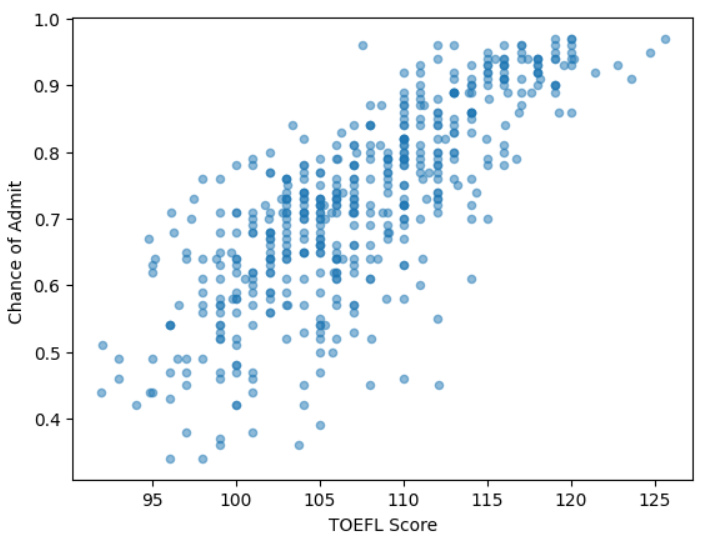
\includegraphics[width=0.9\textwidth]{../figures/scatter_toefl_admit.png}
	\caption{Relation entre TOEFL Score et Chance of Admit}
	\label{fig:scatter_toefl_admit}
\end{figure}

Tendance similaire : TOEFL élevé → chance d’admission élevée. Lignes verticales indiquent plusieurs étudiants ayant le même score.

\subsection{Chance of Admit par expérience de recherche}
Boîte à moustaches (\textbf{Figure 1.13}).

\begin{figure}[!htbp]
	\centering
	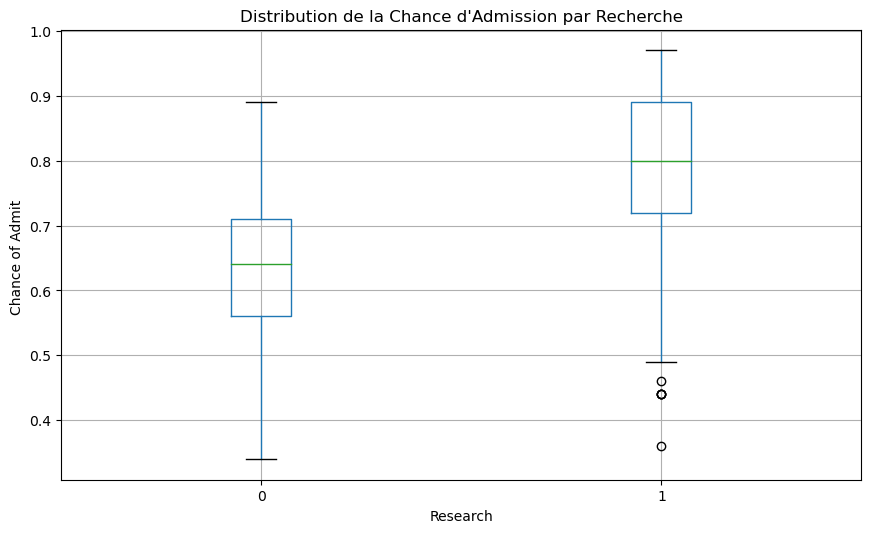
\includegraphics[width=0.9\textwidth]{../figures/distribution_par_search.png}
	\caption{Chance of Admit en fonction de l’expérience de recherche}
	\label{fig:boxplot_research_admit}
\end{figure}

Différence nette :
\begin{itemize}
	\item Sans recherche (0) : médiane ≈ 0.65
	\item Avec recherche (1) : médiane ≈ 0.8, 3ème quartile ≈ 0.89
\end{itemize}

\subsection{Distribution du TOEFL selon University Rating}
\begin{figure}[!htbp]
	\centering
	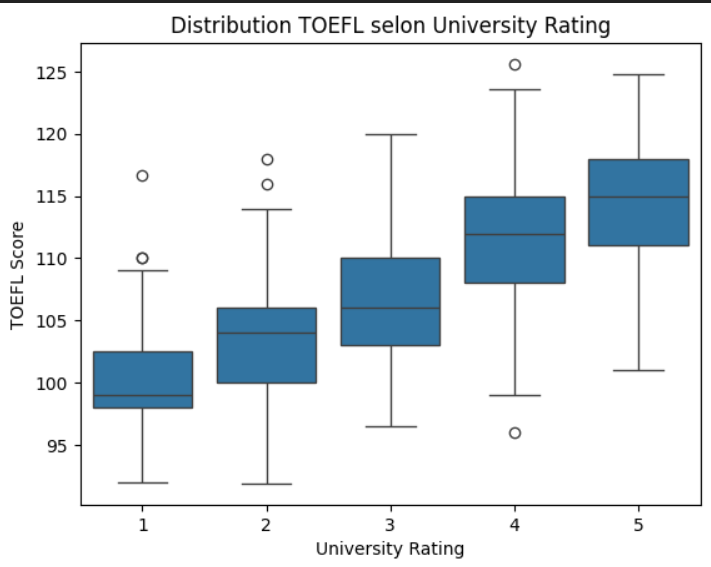
\includegraphics[width=0.9\textwidth]{../figures/TU.png}
	\caption{Distribution du TOEFL selon University Rating}
	\label{fig:TOEFLtoUR}
\end{figure}

Universités mieux classées (4-5) → scores TOEFL plus élevés, corrélation positive.

\subsection{Nombre de candidats selon expérience de recherche}
Histogramme (\textbf{Figure 1.15}).

\begin{figure}[!htbp]
	\centering
	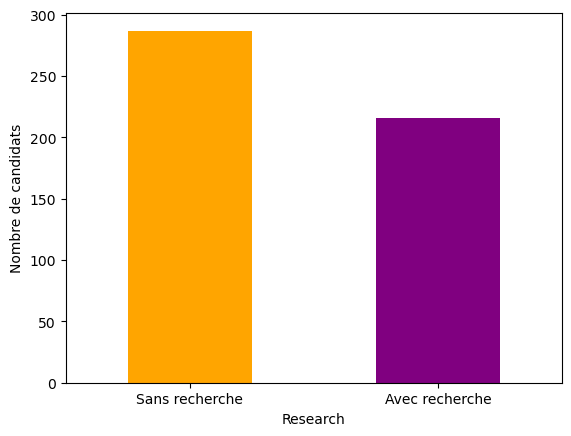
\includegraphics[width=0.9\textwidth]{../figures/nbr_selon_search.png}
	\caption{Répartition des candidats avec ou sans expérience de recherche}
	\label{fig:bar_research_counts}
\end{figure}

Environ 250-300 candidats sans expérience et 200-250 avec expérience.

\section{Conclusion de l'exploration}

Cette exploration met en évidence :
\begin{itemize}
	\item Corrélation positive entre GRE, TOEFL, CGPA et chance d’admission ;
	\item Influence de l’expérience de recherche sur la probabilité d’admission ;
	\item Distribution relativement équilibrée avec certaines zones de concentration.
\end{itemize}

Ces observations guideront les choix de modélisation dans les sections suivantes.

\chapter{Modélisation}

Dans cette section, nous avons testé plusieurs algorithmes de classification afin de prédire la probabilité d’admission des candidats. 
Les modèles utilisés sont : \textbf{SVM (SVC)}, \textbf{Arbre de décision}, \textbf{Forêt aléatoire}, \textbf{Régression logistique} et \textbf{K plus proches voisins (KNN)}. 
Pour chaque modèle, nous avons appliqué une normalisation des données avec \texttt{StandardScaler} et utilisé un pipeline pour enchaîner les étapes.

\section{Évaluation des modèles}
Chaque modèle a été entraîné sur $80\%$ des données et testé sur $20\%$. Les métriques utilisées pour comparer les performances sont :
\begin{itemize}
    \item \textbf{Accuracy} : proportion de prédictions correctes.
    \item \textbf{Precision} : proportion de vrais positifs parmi les positifs prédits.
    \item \textbf{Recall} : proportion de vrais positifs correctement détectés.
    \item \textbf{F1-score} : moyenne harmonique entre précision et rappel.
\end{itemize}

\section{Résultats comparatifs}
Les performances globales sont résumées dans le tableau suivant :

\begin{table}[H]
\centering
\begin{tabular}{lcccc}
\hline
\textbf{Modèle} & \textbf{Accuracy} & \textbf{Précision} & \textbf{Rappel} & \textbf{F1-score} \\
\hline
SVC & 0.90 & 0.94 & 0.91 & 0.92 \\
Arbre de décision & 0.76 & 0.82 & 0.82 & 0.82 \\
Forêt aléatoire & 0.87 & 0.89 & 0.93 & 0.91 \\
Régression logistique & 0.87 & 0.92 & 0.88 & 0.90 \\
KNN & 0.87 & 0.92 & 0.88 & 0.90 \\
\hline
\end{tabular}
\caption{Comparaison des performances des différents modèles.}
\end{table}

\section{Courbes d'apprentissage}
Pour mieux comprendre le biais et la variance de chaque modèle, nous avons tracé les courbes d'apprentissage. Ces dernières montrent l’évolution de la performance en fonction de la taille de l’échantillon d’entraînement.

\begin{figure}[H]
    \centering
    
\includegraphics[width=0.7\textwidth]{figures/learning_curve_svc.png}
    \caption{Courbe d’apprentissage pour SVC.}
\end{figure}

\begin{figure}[H]
    \centering
    
\includegraphics[width=0.7\textwidth]{figures/learning_curve_rf.png}
    \caption{Courbe d’apprentissage pour Forêt aléatoire.}
\end{figure}

\begin{figure}[H]
    \centering
    
\includegraphics[width=0.7\textwidth]{figures/learning_curve_dtc.png}
    \caption{Courbe d’apprentissage pour Arbre de décision.}
\end{figure}

\begin{figure}[H]
    \centering
    
\includegraphics[width=0.7\textwidth]{figures/learning_curve_lr.png}
    \caption{Courbe d’apprentissage pour Régression logistique.}
\end{figure}

\begin{figure}[H]
    \centering
    
\includegraphics[width=0.7\textwidth]{figures/learning_curve_knn.png}
    \caption{Courbe d’apprentissage pour KNN.}
\end{figure}

\section{Discussion}
L’analyse comparative montre que : 
\begin{itemize}
    \item Le modèle \textbf{SVC} obtient la meilleure performance globale avec un F1-score de 0.92, grâce à une bonne précision et un bon rappel.
    \item Les modèles \textbf{Forêt aléatoire} et \textbf{KNN} présentent des résultats proches (accuracy de 0.87 et F1-score de 0.90). 
    \item L’\textbf{arbre de décision}, en revanche, a un score plus faible (accuracy 0.76), et tend à sur-apprendre les données d’entraînement (overfitting).
    \item La \textbf{régression logistique} se démarque car, contrairement aux modèles comme l’arbre de décision, la forêt aléatoire ou KNN qui mémorisent fortement les données, elle parvient à \textbf{apprendre une véritable relation généralisable entre les variables et la probabilité d’admission}. 
\end{itemize}

Ainsi, même si SVC donne les meilleurs résultats en termes de F1-score, la régression logistique apparaît comme un modèle plus robuste et interprétable pour ce type de problématique. Elle a donc été retenue et sauvegardée pour de futures prédictions.

\chapter{Déploiement}

Dans ce chapitre, nous présentons la manière dont le modèle entraîné peut être testé par un utilisateur.

\section{Test interactif du modèle}
Un script Python a été développé pour permettre à l'utilisateur d'entrer ses informations académiques et personnelles afin d'obtenir une prédiction de réussite au concours d'entrée universitaire.

\begin{itemize}
    \item L'utilisateur renseigne le \textbf{GRE Score}, \textbf{TOEFL Score}, \textbf{Note de l'université}, \textbf{SOP}, \textbf{LOR}, \textbf{CGPA} et l'expérience de \textbf{recherche}.
    \item Pour chaque entrée, si l'utilisateur n'a pas de donnée, une valeur par défaut neutre est utilisée.
    \item Le script affiche ensuite le résultat de la prédiction : 
    \begin{itemize}
        \item \texttt{Candidat probablement admis} si le modèle prédit 1.
        \item \texttt{Candidat probablement non admis} si le modèle prédit 0.
    \end{itemize}
\end{itemize}

\section{Chargement du modèle}
Le modèle a été sauvegardé à l'aide de la librairie \texttt{pickle} et peut être chargé depuis le fichier \texttt{logistic.pkl} pour être utilisé dans le script de test.

\section{Illustration du script}
\begin{verbatim}
import pickle as pkl
with open('models/logistic.pkl', 'rb') as f:
    model_loaded = pkl.load(f)

test_model_input(model_loaded)
\end{verbatim}

Ce script représente une première étape de déploiement dans un environnement local et permet de vérifier le fonctionnement du modèle avant tout déploiement plus complexe.

\chapter*{Conclusion}
\addcontentsline{toc}{chapter}{Conclusion}

Ce travail de recherche nous a permis d'aboutir à la création et à la validation d'un modèle prédictif dont l'objectif principal est d'évaluer les chances d’admission d’un étudiant, en s’appuyant sur le dataset. La méthodologie adoptée repose sur une succession d'étapes clés :

\begin{itemize}
	\item \textbf{Prédiction en pourcentage} : Avant toute classification binaire, nous avons utilisé la \textbf{régression linéaire} pour estimer la probabilité d’admission d’un étudiant. Cette approche fournit une valeur continue interprétable entre 0 et 1, offrant une vision quantitative des chances d’admission. Elle permet ainsi de mieux guider l’utilisateur et de compléter les décisions binaires.
	
	\item \textbf{Préparation des données} : Cette phase préliminaire, souvent sous-estimée, s’est avérée déterminante. Elle a inclus le nettoyage des données, leur exploration approfondie, et la sélection des variables principales pour la prédiction.
	
	\item \textbf{Modélisation et classification} : Une comparaison approfondie parmi plusieurs algorithmes d’apprentissage supervisé a été réalisée. Nous avons confronté les performances du \textbf{SVC}, \textbf{Random Forest}, \textbf{Arbre de Décision}, \textbf{Régression Logistique} et \textbf{K Nearest Neighbors}, afin de déterminer lequel de ces algorithmes était le plus précis et adapté à notre problématique. La régression logistique, en particulier, a été utilisée pour produire la décision binaire (admis / non admis).
	
	\item \textbf{Évaluation} : Au-delà des métriques classiques de performance comme l’exactitude, la précision ou le score F1, nous avons analysé les courbes d’apprentissage pour détecter et comprendre les écueils classiques que sont le surajustement ou le sous-ajustement, garantissant ainsi la robustesse de notre modèle.
	
	\item \textbf{Déploiement} : Pour concrétiser cette étude, une application interactive a été développée. Elle permet à un utilisateur de saisir ses informations et d’obtenir non seulement la décision binaire grâce à la régression logistique, mais également une estimation du \textbf{pourcentage de chances d’admission} fournie par la régression linéaire. Cette double approche offre à l’utilisateur une vision plus complète et personnalisée.
\end{itemize}

L’examen méticuleux des performances a révélé que la \textbf{Régression Logistique} s’est imposée comme l’approche la plus pertinente pour notre jeu de données. Son excellence réside dans son équilibre et sa remarquable capacité à généraliser, évitant ainsi les pièges du surajustement dans lesquels certains concurrents sont tombés. Parallèlement, le modèle de \textbf{régression linéaire} a permis de quantifier les probabilités d’admission, donnant un indicateur continu et interprétable.

Enfin, ce mémoire ne se contente pas de présenter un modèle opérationnel ; il ouvre la voie à de multiples prolongements. Le développement d’une interface web intuitive ou la publication sous forme d’API constituent des évolutions naturelles pour étendre la portée de cet outil.  

\bigskip
Cette recherche rappelle également que la performance d’un modèle de machine learning ne naît pas de la sophistication de l’algorithme, mais bien de la qualité du travail en amont : la préparation des données et leur analyse critique restent la pierre angulaire de tout projet réussi en science des données.

\chapter*{Annexes}
\addcontentsline{toc}{chapter}{Annexes}

\section*{Bibliothèques utilisées pour l'EDA}
\begin{figure}[H]
	\centering
	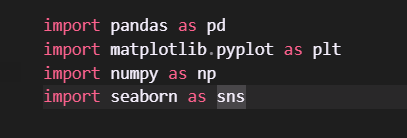
\includegraphics[width=0.7\textwidth]{../figures/importation_01.png}
\end{figure}
\noindent \textbf{Explication :} 
\texttt{pandas} pour la manipulation des données, 
\texttt{matplotlib} et \texttt{seaborn} pour la visualisation graphique, 
\texttt{numpy} pour les calculs numériques.

\section*{Chargement du dataset}
\begin{figure}[H]
	\centering
	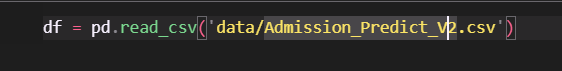
\includegraphics[width=0.7\textwidth]{../figures/load_dataset.png}
\end{figure}
\noindent \textbf{Explication :} 
La fonction \texttt{pd.read\_csv()} permet de charger le dataset afin de l’exploiter pour l’analyse et la modélisation.

\section*{Affichage des premières lignes du dataset}
\begin{figure}[H]
	\centering
	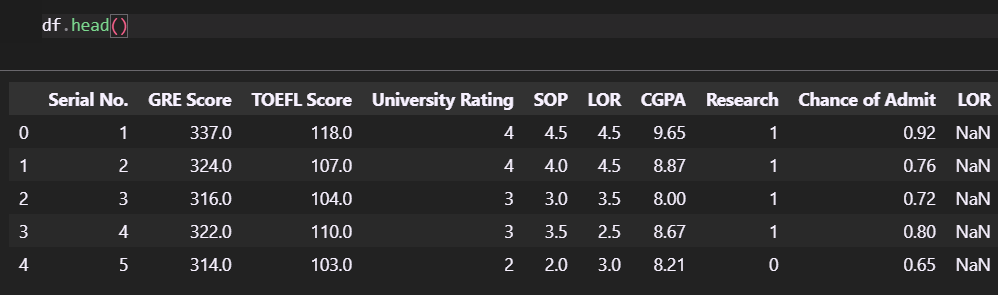
\includegraphics[width=0.9\textwidth]{../figures/head_5}
\end{figure}
\noindent \textbf{Explication :} 
La méthode \texttt{df.head()} affiche les cinq premières lignes du dataset pour un aperçu rapide de sa structure.

\section*{Aperçu du type des données}
\begin{figure}[H]
	\centering
	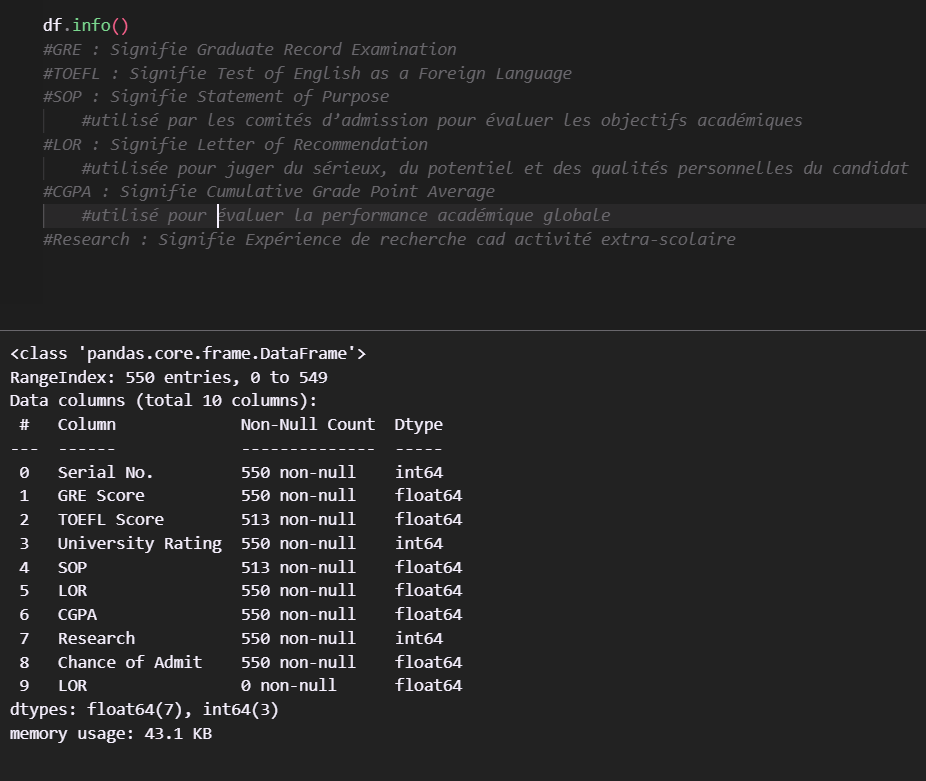
\includegraphics[width=0.9\textwidth]{../figures/info_dataset.png}
\end{figure}
\noindent \textbf{Explication :} 
\texttt{df.info()} fournit un résumé des types de données et du nombre de valeurs non nulles par colonne.

\section*{Résumé statistique du dataset}
\begin{figure}[H]
	\centering
	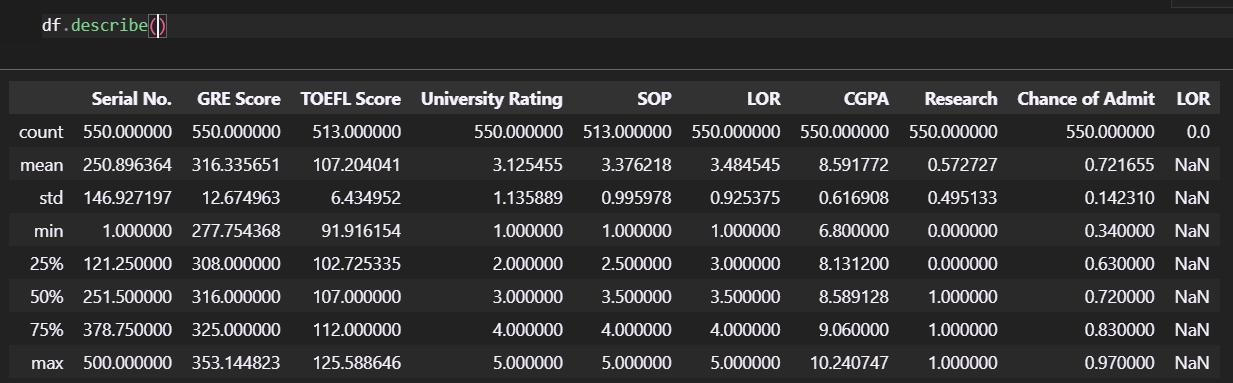
\includegraphics[width=0.9\textwidth]{../figures/describe_dataset.png}
\end{figure}
\noindent \textbf{Explication :} 
\texttt{df.describe()} calcule des statistiques descriptives : moyenne, écart-type, valeurs minimales et maximales.

\section*{Suppression des colonnes inutiles}
\begin{figure}[H]
	\centering
	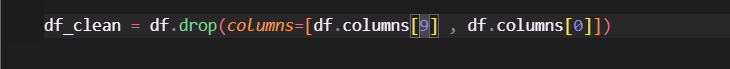
\includegraphics[width=0.9\textwidth]{../figures/remove_c.png}
\end{figure}
\noindent \textbf{Explication :} 
La colonne \texttt{Serial No.} et le doublon \texttt{LOR} ont été supprimés car non pertinents pour l’analyse.

\section*{Nettoyage des données}
\begin{figure}[H]
	\centering
	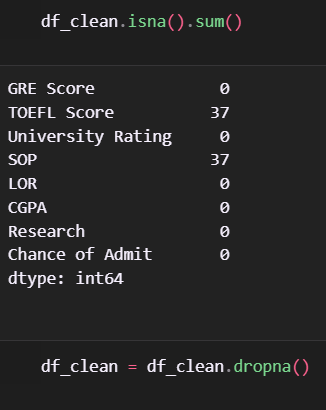
\includegraphics[width=0.9\textwidth]{../figures/cleaning_d.png}
\end{figure}
\noindent \textbf{Explication :} 
\texttt{df\_clean.isna().sum()} permet de compter les valeurs manquantes.  
Elles ont ensuite été supprimées avec \texttt{df\_clean.dropna()}.

\section*{Visualisation univariée des données}
\begin{figure}[H]
	\centering
	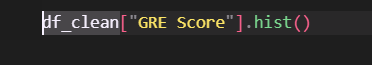
\includegraphics[width=0.9\textwidth]{../figures/v1.png}
	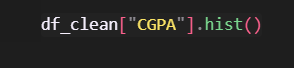
\includegraphics[width=0.9\textwidth]{../figures/v2.png}
	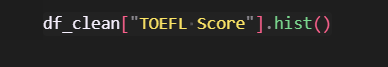
\includegraphics[width=0.9\textwidth]{../figures/v3.png}
	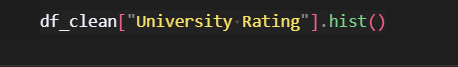
\includegraphics[width=0.9\textwidth]{../figures/v4.png}
	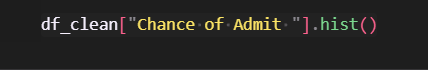
\includegraphics[width=0.9\textwidth]{../figures/v5.png}
	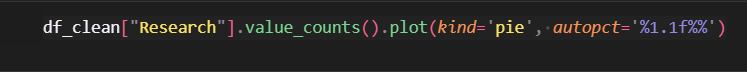
\includegraphics[width=0.9\textwidth]{../figures/v6.png}
\end{figure}
\noindent \textbf{Explication :} 
Ces codes présentent la distribution de chaque variable individuelle.

\section*{Visualisation bivariée des données}
\begin{figure}[H]
	\centering
	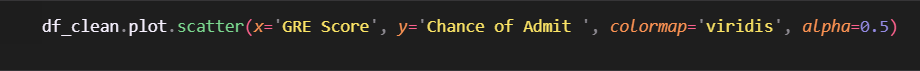
\includegraphics[width=0.9\textwidth]{../figures/b1.png}
	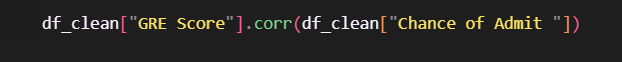
\includegraphics[width=0.9\textwidth]{../figures/b2.png}
	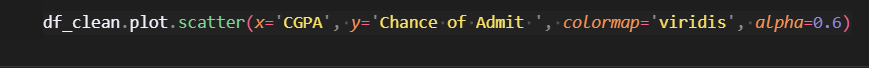
\includegraphics[width=0.9\textwidth]{../figures/b3.png}
	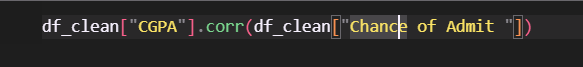
\includegraphics[width=0.9\textwidth]{../figures/b4.png}
	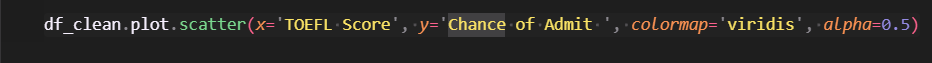
\includegraphics[width=0.9\textwidth]{../figures/b5.png}
	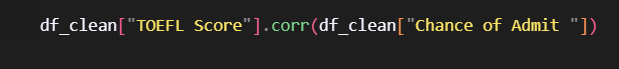
\includegraphics[width=0.9\textwidth]{../figures/b6.png}
	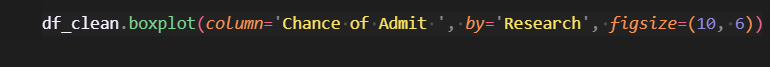
\includegraphics[width=0.9\textwidth]{../figures/b7.png}
	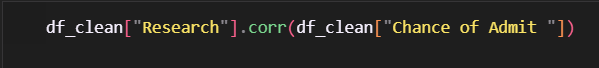
\includegraphics[width=0.9\textwidth]{../figures/b8.png}
	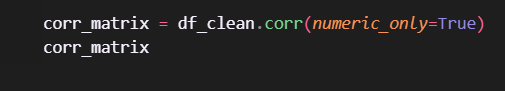
\includegraphics[width=0.9\textwidth]{../figures/b9.png}
	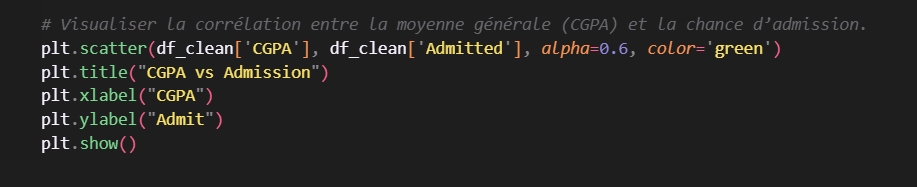
\includegraphics[width=0.9\textwidth]{../figures/b10.png}
	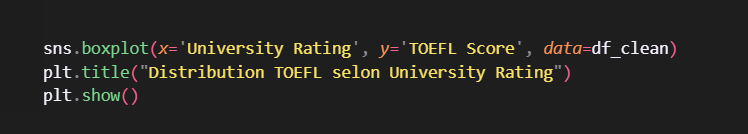
\includegraphics[width=0.9\textwidth]{../figures/b11.png}
	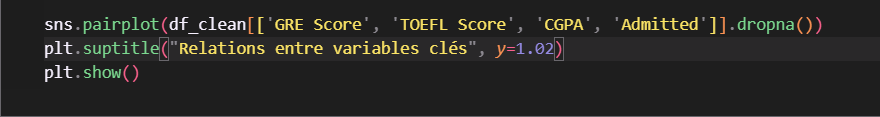
\includegraphics[width=0.9\textwidth]{../figures/b12.png}
\end{figure}
\noindent \textbf{Explication :} 
Ces codes montrent les relations entre deux variables, utiles pour détecter corrélations et tendances.

\section*{Variables utilisées pour l’entraînement du modèle (régression)}
\begin{figure}[H]
	\centering
	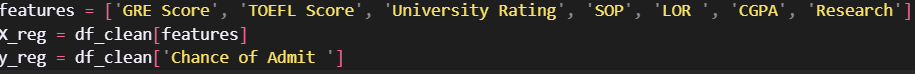
\includegraphics[width=0.9\textwidth]{../figures/regression.png}
\end{figure}

\section*{Variables utilisées pour l’entraînement du modèle (classification)}
\begin{figure}[H]
	\centering
	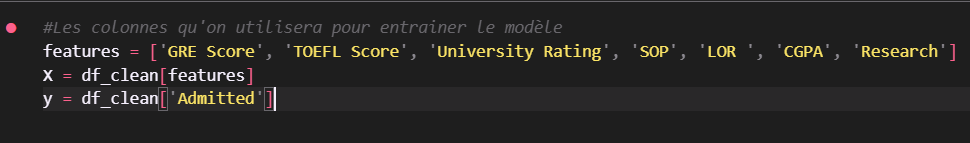
\includegraphics[width=0.9\textwidth]{../figures/v_u.png}
\end{figure}

\section*{Bibliothèques utilisées pour l’entraînement du modèle}
\begin{figure}[H]
	\centering
	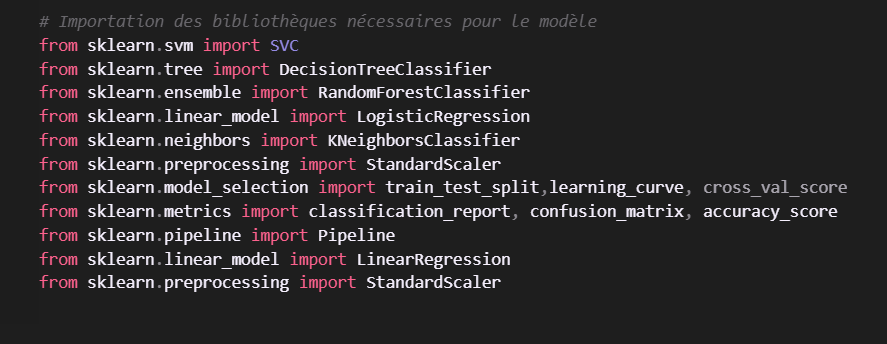
\includegraphics[width=0.9\textwidth]{../figures/b_u.png}
\end{figure}
\noindent \textbf{Imports principaux :}
\begin{itemize}
	\item \texttt{from sklearn.svm import SVC} : Support Vector Classifier.  
	\item \texttt{from sklearn.tree import DecisionTreeClassifier} : Arbre de décision.  
	\item \texttt{from sklearn.ensemble import RandomForestClassifier} : Forêt aléatoire.  
s	\item \texttt{from sklearn.linear_model import LogisticRegression, LinearRegression} : Régression logistique et linéaire.  
	\item \texttt{from sklearn.neighbors import KNeighborsClassifier} : K plus proches voisins.  
	\item \texttt{from sklearn.preprocessing import StandardScaler} : Normalisation des données.  
	\item \texttt{from sklearn.model_selection import train\_test\_split, learning\_curve, cross\_val\_score} : Division données et validation croisée.  
	\item \texttt{from sklearn.metrics import classification\_report, confusion\_matrix, accuracy\_score} : Métriques d’évaluation.  
	\item \texttt{from sklearn.pipeline import Pipeline} : Chaîne de traitement complète.  
s\end{itemize}

\section*{Exemple de code utilisé pour l’entraînement du modèle}
\begin{figure}[H]
	\centering
	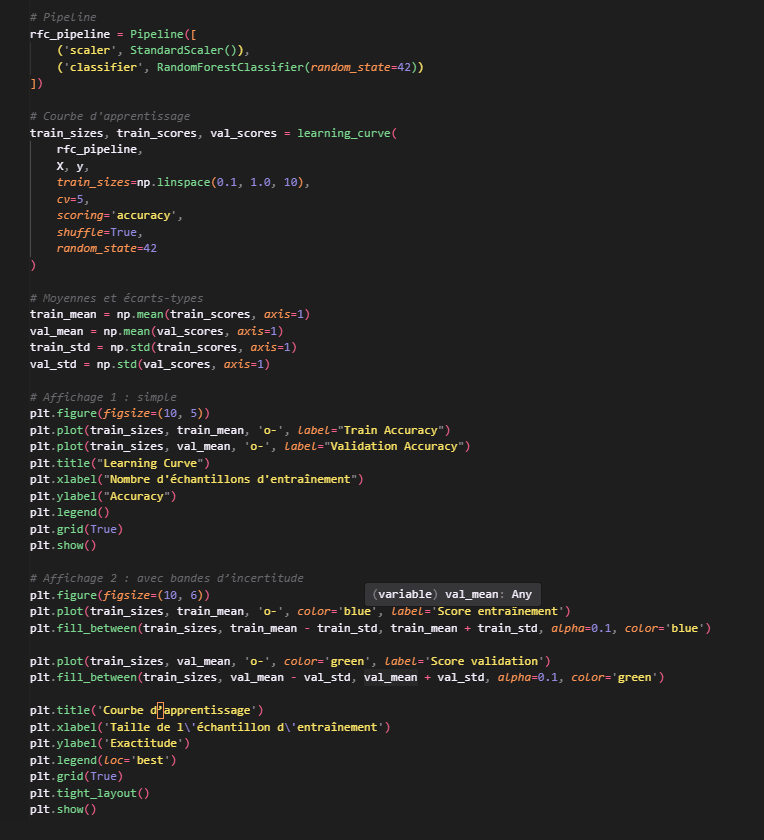
\includegraphics[width=0.9\textwidth]{../figures/E_u_t.png}
\end{figure}

\section*{Exemple de code utilisé pour tester le modèle}
\begin{figure}[H]
	\centering
	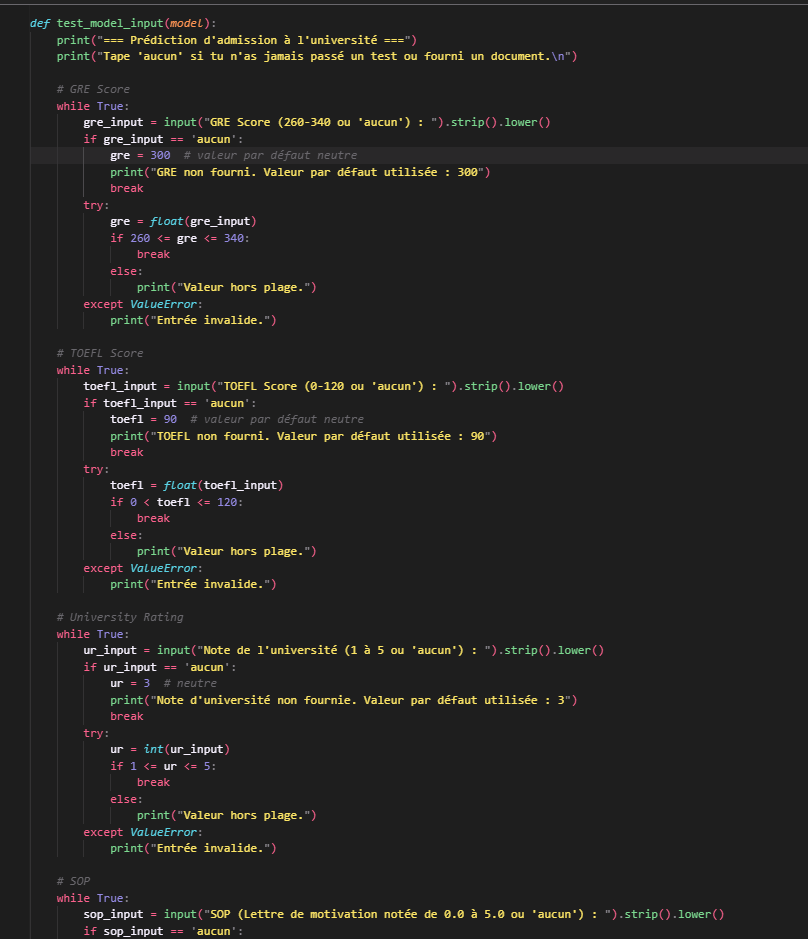
\includegraphics[width=0.9\textwidth]{../figures/t1.png}
	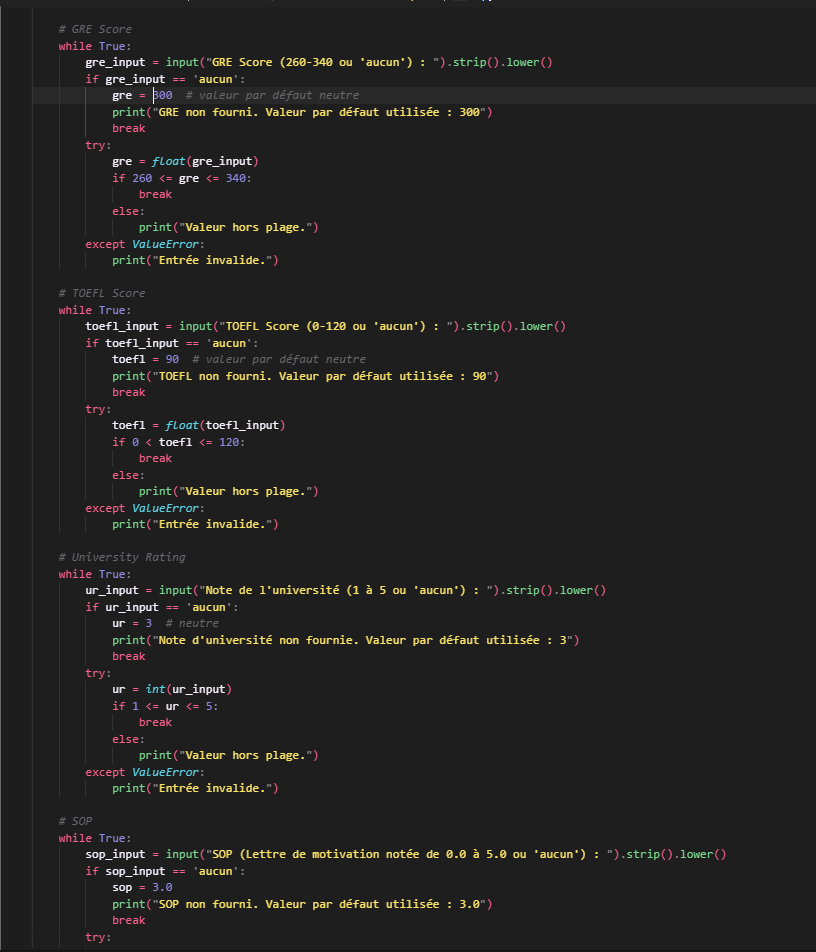
\includegraphics[width=0.9\textwidth]{../figures/t2.png}
	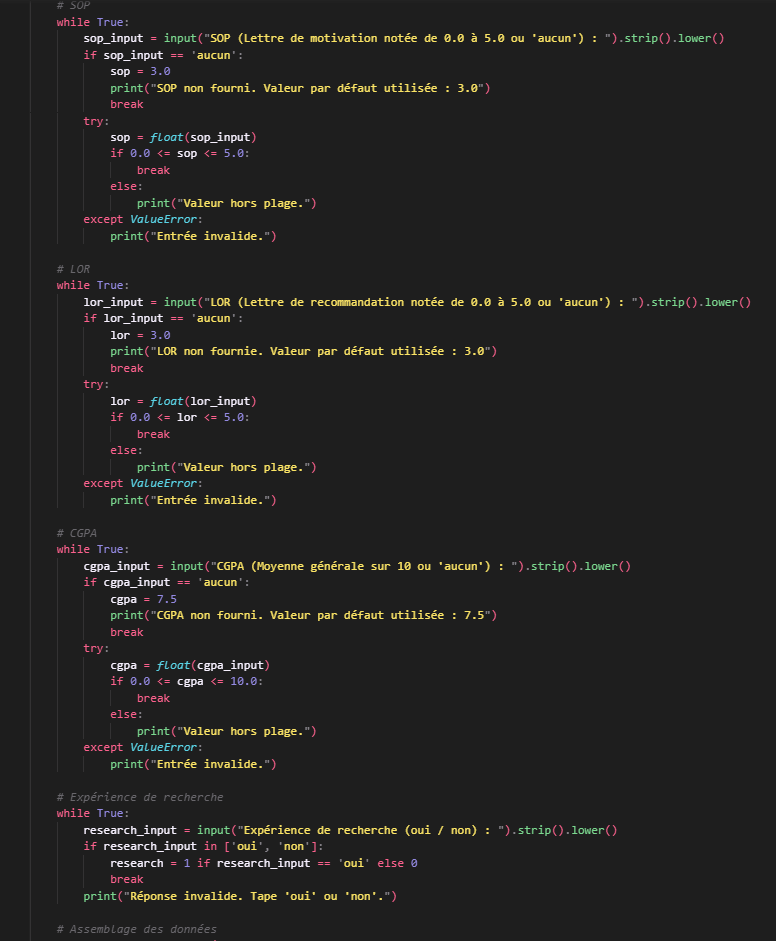
\includegraphics[width=0.9\textwidth]{../figures/t3.png}
	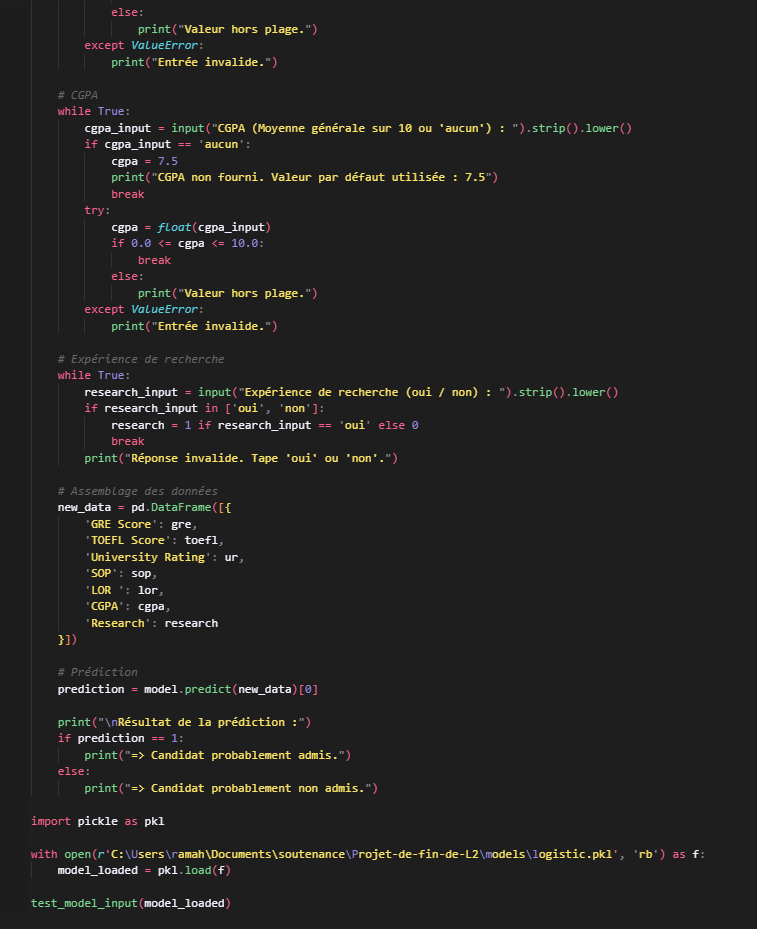
\includegraphics[width=0.9\textwidth]{../figures/t4.png}
\end{figure}
\noindent \textbf{Explication :} 
Ces extraits montrent l’évaluation du modèle sur le dataset de test, incluant la prédiction et l’analyse des performances.

\chapter*{Bibliographie}
\addcontentsline{toc}{chapter}{Bibliographie}

\begin{itemize}
	% === DATASETS ===
	\item \textbf{Dataset principal} : \textit{admission\_rate\_ver\_1.csv}. \\
	Disponible sur : \url{https://dr-raz.org/statistical-literacy-csv-data}. \\
	Consulté le 25 août 2025.
	
	\item \textbf{Dataset test} : \textit{gc\_data.csv}. \\
	Disponible sur : \url{http://sourceforge.net/projects/triangleinequal/files/Grad%20Cafe%20Data/gc_data.csv/download}. \\
	Consulté le 20 août 2025.
	
	\item \textbf{Dataset test} : \textit{Predict students dropout and academic success}. \\
	Disponible sur : \url{https://archive.ics.uci.edu/dataset/697/predict+students+dropout+and+academic+success}. \\
	Consulté le 18 août 2025.
	
	\item \textbf{Dataset test} : \textit{Graduate school admission data}. \\
	Disponible sur : \url{https://figshare.com/articles/dataset/Graduate_school_admission_data/19561582}. \\
	Consulté le 22 août 2025.
	
	\item \textbf{TheGradCafe} : \textit{How to scrape the website of thegradcafe}. \\
	Disponible sur : \url{https://forum.thegradcafe.com/topic/51483-scraped-admissions-data}. \\
	Consulté le 21 août 2025.
	
	% === CONCEPTS STAT ET ML ===
	\item \textbf{Régression linéaire}. Disponible sur : \url{https://fr.wikipedia.org/wiki/R%C3%A9gression_lin%C3%A9aire}. Consulté le 1 septembre 2025.
	
	\item \textbf{Classification}. Disponible sur : \url{https://fr.wikipedia.org/wiki/Classification_(statistiques)}. Consulté le 1 septembre 2025.
	
	\item \textbf{Régression logistique}. Disponible sur : \url{https://fr.wikipedia.org/wiki/R%C3%A9gression_logistique}. Consulté le 1 septembre 2025.
	
	\item \textbf{Arbre de décision (Decision Tree)}. Disponible sur : \url{https://fr.wikipedia.org/wiki/Arbre_de_d%C3%A9cision}. Consulté le 1 septembre 2025.
	
	\item \textbf{Support Vector Machine (SVC)}. Disponible sur : \url{https://fr.wikipedia.org/wiki/Machine_%C3%A0_vecteurs_de_support}. Consulté le 1 septembre 2025.
	
	\item \textbf{Hyperplan}. Disponible sur : \url{https://fr.wikipedia.org/wiki/Hyperplan}. Consulté le 1 septembre 2025.
	
	\item \textbf{KNN (K Nearest Neighbors)}. Disponible sur : \url{https://fr.wikipedia.org/wiki/M%C3%A9thode_des_k_plus_proches_voisins}. Consulté le 1 septembre 2025.

	\item \textbf{Valeurs manquantes}. Disponible sur : \url{https://fr.wikipedia.org/wiki/Imputation_en_statistique}. Consulté le 1 septembre 2025.
	
	\item \textbf{Validation croisée (Score validation)}. Disponible sur : \url{https://fr.wikipedia.org/wiki/Validation_crois%C3%A9e_(statistiques)}. Consulté le 1 septembre 2025.
	
	\item \textbf{Variable quantitative}. Disponible sur : \url{https://fr.wikipedia.org/wiki/Variable_al%C3%A9atoire}. Consulté le 1 septembre 2025.
	
	\item \textbf{Variable discrète}. Disponible sur : \url{https://fr.wikipedia.org/wiki/Variable_al%C3%A9atoire#Variables_discr%C3%A8tes}. Consulté le 1 septembre 2025.
	
	\item \textbf{Variable cible}. Disponible sur : \url{https://fr.wikipedia.org/wiki/Variable_d%C3%A9pendante}. Consulté le 1 septembre 2025.
	
	
	\item \textbf{Web scraping (Scraper)}. Disponible sur : \url{https://fr.wikipedia.org/wiki/Web_scraping}. Consulté le 1 septembre 2025.
	
	\item \textbf{Courbe d’apprentissage}. Disponible sur : \url{https://en.wikipedia.org/wiki/Learning_curve}. Consulté le 1 septembre 2025.
	
	\item \textbf{Modèle prédictif}. Disponible sur : \url{https://fr.wikipedia.org/wiki/Mod%C3%A8le_pr%C3%A9dictif}. Consulté le 1 septembre 2025.
	
	\item \textbf{Surapprentissage}. Disponible sur : \url{https://fr.wikipedia.org/wiki/Surapprentissage}. Consulté le 1 septembre 2025.
	
	% === BIBLIOTHÈQUES PYTHON ===
	\item \textbf{Pandas}. Disponible sur : \url{https://fr.wikipedia.org/wiki/Pandas_(logiciel)}. Consulté le 1 septembre 2025.
	
	\item \textbf{Matplotlib}. Disponible sur : \url{https://fr.wikipedia.org/wiki/Matplotlib}. Consulté le 1 septembre 2025.
	
	\item \textbf{Seaborn}. Disponible sur : \url{https://seaborn.pydata.org/}. Consulté le 1 septembre 2025.
	
	\item \textbf{NumPy}. Disponible sur : \url{https://fr.wikipedia.org/wiki/NumPy}. Consulté le 1 septembre 2025.
	
	\item \textbf{Scikit-learn}. Disponible sur : \url{https://fr.wikipedia.org/wiki/Scikit-learn}. Consulté le 1 septembre 2025.
	
	\item \textbf{StandardScaler}. Disponible sur : \url{https://scikit-learn.org/stable/modules/generated/sklearn.preprocessing.StandardScaler.html}. Consulté le 1 septembre 2025.
	
	\item \textbf{Train-test split}. Disponible sur : \url{https://scikit-learn.org/stable/modules/cross_validation.html#cross-validation}. Consulté le 1 septembre 2025.
	
	% === METRIQUES ===
	\item \textbf{Accuracy}. Disponible sur : \url{https://fr.wikipedia.org/wiki/Pr%C3%A9cision_et_rappel}. Consulté le 1 septembre 2025.
	
	\item \textbf{Precision}. Disponible sur : \url{https://fr.wikipedia.org/wiki/Pr%C3%A9cision_et_rappel}. Consulté le 1 septembre 2025.
	
	\item \textbf{Recall}. Disponible sur : \url{https://fr.wikipedia.org/wiki/Pr%C3%A9cision_et_rappel}. Consulté le 1 septembre 2025.
	
	\item \textbf{F1-score}. Disponible sur : \url{https://fr.wikipedia.org/wiki/F-mesure}. Consulté le 1 septembre 2025.
	
	\item \textbf{Kaggle}. Disponible sur : \url{https://fr.wikipedia.org/wiki/Kaggle}. Consulté le 1 septembre 2025.
\end{itemize}


\end{document}
